\startdocument 

\section{Moduli}
\label{ModuliSection}

\subsection{String Compactifications}

Even if a full non-perturbative understanding of string and M-theory is still lacking, it has long been understood that at low energies there are 5
different limits of string theory in 10-dimensional flat space, which are related to each other by duality transformations. 
The M-theory picture also leads to a sixth limit, namely 11-dimensional supergravity, often referred to as the low-energy limit of M-theory, the still-not-fully-defined theory that encompasses all the string theories as different limits. 

What these limits have in common, and arguably the \emph{single most important physical implication of string theories}, is the existence of extra dimensions. The process of starting from a higher-dimensional theory and then obtaining a 4-dimensional effective theory is known as compactification, and over the past 35 years string compactifications have been studied in much detail. Starting from a 10-dimensional theory, the different fields have to be decomposed into their components in the 4 non-compact dimensions and also their ones in the extra compact dimensions. For instance, the 10-dimensional graviton $ g_{_{MN}} $ splits into the 4-dimensional graviton $g_{\mu\nu}$, a set of scalar fields $g_{mn}$ that correspond to moduli fields and potentially also vector fields $g_{\mu n}$. Notice that from the 4-dimensional perspective the indices $m,n$ are just internal indices, as in compactification the extra dimensions are regarded as no longer directly visible from the 4-dimensional perspective:
\begin{equation}
g_{_{MN}}=\begin{pmatrix} g_{\mu\nu} & g_{\mu n} \\
g_{n\nu} & g_{mn}
\end{pmatrix}\qquad \mu,\nu =1, \cdots, 4\ ; \qquad m,n=1,\cdots, 6
\end{equation}
A similar decomposition is performed with the higher-form antisymmetric tensors $B_{MN}$, $C_{MNP}$, etc present in each of the 6 theories, with the form content of each theory shown in Tab. \ref{tab:boson_spectrum}.

\begin{table}[H]
\begin{center}
\centering
\begin{tabular}{ | c | c | c | c | }
\hline
\cellcolor[gray]{0.9}  {\bf Theory} &  \cellcolor[gray]{0.9} {\bf Dimension } &  \cellcolor[gray]{0.9} {\bf Supercharges} &  \cellcolor[gray]{0.9} {\bf Massless Bosons}   \\
\hline \hline 
{Heterotic}   & 10  & 16  & $g_{_{MN}}, B_{_{MN}}, \phi $  \\
$E_8 \times E_8$ & & &$A_{_M}^{ij}$ \\
\hline
{Heterotic}   & 10  & 16  & $g_{_{MN}}, B_{_{MN}}, \phi $  \\
$SO(32)$ & & &$A_{_M}^{ij}$ \\
\hline
{Type I}   & 10  & 16  & $g_{_{MN}},  \phi, A_{_M}^{ij} $  \\
$SO(32)$ & & &$C_{_{MN}}$ \\
\hline
{Type IIA}   & 10  & 32  & $g_{_{MN}}, B_{_{MN}}, \phi $  \\
& & &$C_{_M}, C_{_{MNP}}$ \\
\hline
{Type IIB}   & 10  & 32  & $g_{_{MN}}, B_{_{MN}},\phi $  \\
& & &$C_{_0}, C_{_{MN}}, C_{_{MNPQ}}$ \\
\hline
{M-Theory}   & 11  & 32  & $g_{_{MN}}, C_{_{MNP}}$ \\
\hline
\end{tabular}
\end{center} 
\caption {\footnotesize{The massless bosonic spectrum of the five string theories and of $11$-dimensional supergravity. The corresponding massless fermionic spectrum is determined by supersymmetry. Moduli fields all originate from these simple spectra in 10d, reduced on the internal manifold. There are also matter states, which in IIA and IIB string theories come from D-brane intersections and in heterotic string theory come from solutions of the Dirac equation with non-trivial gauge configuration. Further moduli, such as open string moduli from separation between D-branes or closed string bundle moduli, can also be present.} }
\label{tab:boson_spectrum}
\end{table}

The most studied compactifications are those that preserve $\cN=1$ supersymmetry. These offer a greater degree of control over the effective action compared to non-supersymmetric theories, while also allowing for the presence of chiral fermions and sufficient dynamics to 
allow for hierarchies and a non-supersymmetric vacuum state.

These correspond in the case of the heterotic or type I theories to the internal space being a Calabi-Yau (CY) manifold. These are manifolds of $SU(3)$ holonomy (or vanishing first Chern class). CY manifolds are complex K\"ahler manifolds, meaning that the metric can be written as a second derivative of a K\"ahler potential $K(z_i, \bar z_{\bar\jmath})$: $g_{i\bar\jmath}=\partial_i\partial_{\bar\jmath} K$. 
However, since they do not have isometries, except for a few numerical examples, there are no known analytic metrics 
for compact CY manifolds of complex dimension greater than one.  Instead, we rely mostly on their topological structure 
(and indeed, the full details of the internal metric are not needed for most parts of the 4-dimensional effective Lagrangian). 
The most relevant topological quantities are the non-trivial homological cycles. 
Their number are given by the corresponding Hodge numbers $h^{p,q}$.  

The simplest CY manifold is the one complex dimensional case corresponding to the torus. This has only two non-trivial homological cycles ($h^{0,1}=h^{1,0}=1$) and its homological structure is summarised by the Hodge diamond:
\bea
\setlength\fboxsep{0.25cm}
\setlength\fboxrule{0.4pt}
\boxed{
\begin{array}{  c  c c}
& h^{1,1}&\\
h^{1,0}& & h^{0,1}\\
& h^{0,0}&
\end{array}
=
\begin{array}{  c  c c}
& 1&\\
1& & 1\\
&1&
\end{array}
}
\nonumber
\eea
Compactifying a string theory on a 2-torus gives rise to two geometric moduli. These are the \emph{K\"ahler modulus} $T$ and the \emph{complex structure modulus} $U$ corresponding to 
\be
\setlength\fboxsep{0.25cm}
\setlength\fboxrule{0.4pt}
\boxed{
T=\sqrt{g}+i B_{12}, \qquad U=\frac{\sqrt{g}}{g_{22}}+i\, \frac{g_{12}}{g_{22}},
}
\ee
where $g_{ij}, B_{ij}$ are the components of the metric and the antisymmetric tensors, with $g ={\rm det} \, g_{ij}$. Roughly speaking, Re $T$ determines the size of the torus and Re $U$ the shape. These simple properties (K\"ahler and complex structure moduli, which respectively correspond to size and shape of the compact space) generalise to the more complicated CY 3-folds and 4-folds which are relevant for string and F-theories. A schematic representation of a Calabi-Yau is figure \ref{Fig:CY2}.


\begin{figure}[t]
\begin{center}
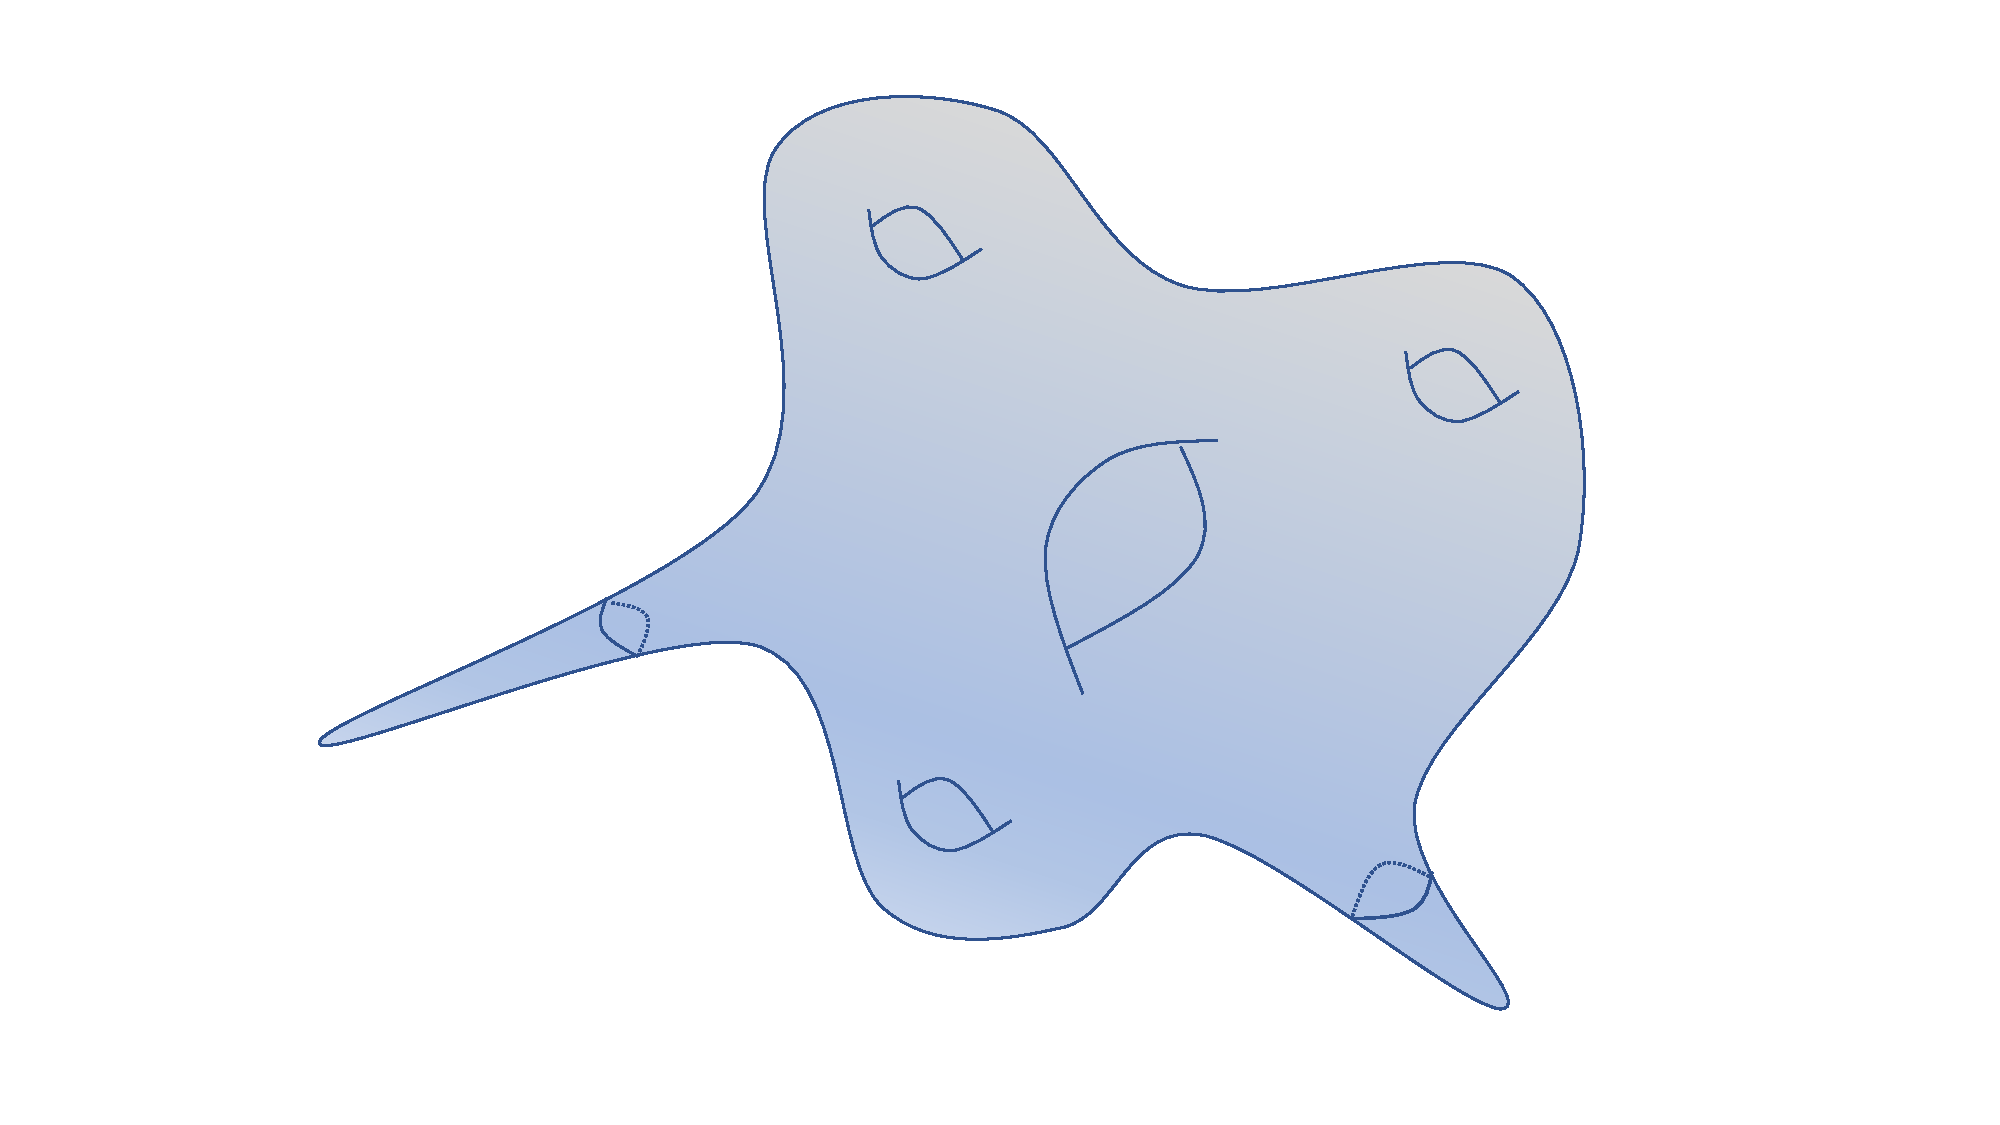
\includegraphics[width=120mm,height=80mm]{Sections/Figures/CalabiYau2.pdf} 
\caption{A schematic representation of the complicated geometry and topology of higher-dimensional Calabi-Yaus.} \label{Fig:CY2} 
\end{center}
\end{figure}

The corresponding Hodge diamond for a 3 complex dimensions CY manifold is:
\bea
\setlength\fboxsep{0.25cm}
\setlength\fboxrule{0.4pt}
\boxed{
\begin{array}{  c  c  c  c  c c c}
& & & h^{3,3} & & &\\
& &  h^{3,2}& & h^{2,3} & &\\
& h^{3,1} & & h^{1,1} & &h^{1,3} &\\
h^{3,0}& & h^{2,1} & & h^{1,2} & & h^{0,3}\\
& h^{2,0} & & h^{2,2} & & h^{0,2} &\\
& & h^{1,0} & & h^{0,1} & &\\
& & & h^{0,0} & & &
\end{array}
=
\begin{array}{  c  c  c  c  c c c}
& & & 1 & & &\\
& & 0 & & 0 & &\\
& 0 & & h^{1,1} & &0 &\\
1& & h^{2,1} & & h^{2,1} & & 1\\
& 0 & & h^{1,1} & &0 &\\
& & 0 & & 0 & &\\
& & & 1 & & &
\end{array}
}
\nonumber
\eea

The relevant numbers here are $h^{1,1}$, counting the number of K\"ahler moduli $T_i, i=1, \cdots, h^{1,1}$ (volumes of 4-cycles or their dual 2-cycles), and $h^{1,2}$, counting the number of complex structure moduli $U_\alpha, \alpha=1,\cdots, h^{1,2}$ (number of 3-cycles). There exist databases of millions of Calabi-Yau manifolds with different values of $h^{1,1}$ and $h^{1,2}$. Typically, these numbers can be as high as hundreds or thousands, see e.g.  \cite{Kreuzer:2000xy}. A recent package, CYTools \cite{Demirtas:2022hqf}, provides tools to compute various topological properties of CY manifolds efficiently.

Another `universal' modulus of great importance is the dilaton $\phi$ (see the table) whose vacuum expectation value $\langle \phi \rangle $ determines the  string coupling, $g_s$. This reflects the fact that string theory has no free parameters and so the strength of string interactions, $g_s$, is itself the expectation value of a field.

In addition to these `universal' moduli, there are also normally other moduli present in the effective theory. These include open string moduli associated to the motion and deformation of branes and corresponding gauge moduli, such as bundle moduli, associated to deformations of vector bundles present in the compactification.

\subsection{General Properties of Moduli}
   
We have said above that the existence of extra dimensions is the most important physical implication of string theory. As moduli are the way these extra dimensions manifest themselves in the 4-dimensional effective field theory, 
moduli are arguably the most important type of particle arising in string compactifications. The 
moduli are scalar degrees of freedom in the effective action of the 4-dimensional observer and describe low energy
excitations in the extra dimensions (such as shape and size of the extra dimensions). They are 
gauge singlet scalars, typically with gravitational strength interactions. In the simplest supersymmetric compactifications with extended supersymmetry, the potential remains flat and the moduli are massless. Besides other issues such as the 
absence of chiral matter, such models are automatically ruled out since these massless moduli would mediate unobserved long-range scalar gravitational-strength interactions (fifth forces).

 Luckily, for models with $\cN= 1$ or $0$ supersymmetry (which, in any case, are the ones of phenomenological interest), there
exist `moduli stabilisation mechanisms'. These lift the flat potentials, give them a mass and allow for the construction of phenomenologically
viable models. Even though moduli are gauge singlets and hard to detect experimentally, their role in string cosmology cannot be over-emphasised. 

Why? Moduli are, in a stringy context, the most natural candidates to be inflaton fields or to drive any alternative early universe cosmology. This is already very important. But what is perhaps even more important, and highly relevant for the later cosmological evolution of the universe, is that in this context the inclusion of moduli into the spectrum has a unique ability to undercut and render invalid the pre-existing cosmology. As we discuss in detail
in chapters \ref{sec:infla}, \ref{reheating} and \ref{sec:DE}, moduli fields can potentially help address many important unanswered questions such as the nature of dark energy, dark matter and dark radiation. 

 Furthermore,  vacuum expectation values of moduli also determine the low energy effective action of a model. As mentioned above, string theory  has no free dimensionless parameters: couplings and ratios of scales in the low energy effective action are set by the 
 values taken on by the moduli. Thus, the task of computing moduli potentials and finding their minima lies at the heart of \emph{string} phenomenology.

 At some levels, moduli are simply examples of scalar fields. The discovery of the existence of an
apparently fundamental scalar (the Higgs) confirms the existence of scalar fields in nature and gives
further motivation for studying their properties. However in many ways, the properties of moduli are crucially different from more familiar scalars such
as the Higgs, and intuitions carried over from the Standard Model electroweak theory or the 
Minimal Supersymmetric Standard Model (MSSM) are misleading when applied to moduli.

Let us list some of these differences:

\begin{itemize}

\item{Moduli are uncharged under Standard Model gauge fields}

It is a basic feature of string moduli that they are neutral under the Standard Model, and also normally under
any additional hidden sector gauge groups that may be introduced. Neutrality under gauge interactions is key to some of the most interesting
features of moduli, as it implies they have no `quick' decay modes.\footnote{In some cases a modulus may be non-linearly charged under an anomalous $U(1)$. This only applies for moduli with shift-symmetries (see below). In this case, the real part of the modulus enters the Fayet-Iliopoulos D-term, and the
axionic part of the modulus is eaten by the massive $U(1)$. The D-term condition then fixes a combination of the real part of the modulus
and the matter fields that are charged under the anomalous $U(1)$, with the orthogonal combination remaining massless.}

\item{The couplings and interactions of moduli come with $\Mp^{-1}$ factors}

Even neutral fields can decay rapidly if they have renormalisable couplings to Standard Model (SM) matter, for example $\Phi h h h$, where $\Phi$ is some modulus field, and $h$ some scalar SM field (such as the Higgs).
However string moduli often descend from higher-dimensional modes of the graviton. This means that all their couplings -- both self-couplings and
couplings the Standard Model sector -- are `really' non-renormalisable.
This includes apparently renormalisable couplings such as
\be
\lambda \,\Phi^4 \in \mc{L}\,.
\ee
In such a coupling, $\lambda$ is dimensionless. However, for moduli $\lambda$ is given by $\frac{m_{\Phi}}{\Mp}$ or $\frac{m_{3/2}}{\Mp}$, where $m_{3/2}$ is the gravitino mass. In this case, $\lambda$ carries hidden factors of $\Mp^{-1}$ and so is numerically extremely small.

The fundamental scale in string theory is the string scale, $M_s$, and not the 4-dimensional Planck scale $\Mp$. In cases
where the string scale and Planck scale are widely separated -- for example with a large compactification volume -- the difference can be significant. Moduli that control local properties of the extra dimensions, such as the size of blow-up cycles, have interactions suppressed by 
the string scale, whereas moduli that control global properties, such as the overall volume, have interactions suppressed by the 4d Planck scale.
Cosmologically it is the latter that are most relevant, as they have the weakest interactions and so survive for the longest time period.

Combined with the neutrality of moduli, the consequence of the $\Mp$ suppression is that moduli always interact weakly. They are hard to produce -- but once produced, they are also hard to get rid of, as they do not thermalise and so live for a long time.

\item{There is generally no concept of `zero VEV' for moduli}

Many scalar fields have a well-defined notion of zero VEV, which acts as a preferred locus in field space. The zero VEV location often
corresponds to the restoration of a broken symmetry. For example, for gauge charged scalars, the gauge symmetry is spontaneously broken for non-zero VEV and restored at zero VEV. An example of this behaviour is the Higgs field, for which the VEV signals electroweak symmetry breaking.

This is not true of moduli. The VEVs of string moduli should instead be interpreted as the values of compactification parameters. For example, the vev of the volume modulus corresponds to the compactification volume (with the canonically normalised field $\Phi$ being defined as $\Phi = - \Mp \ln \mc{V}$) and the VEV of the dilaton corresponds to the string coupling. There is no preferred value for these fields and thus there is no notion of zero VEV for the moduli.\footnote{One can of course define the 'zero vev locus' as the position of the modulus at the full minimum of the potential. However, this is semantics as this locus does not have any \emph{a prior} significance prior to the determination of the potential.} In the low energy theory, the values of these VEVs set the coupling `constants', such as the gauge couplings and the Yukawa couplings.

Note that one exception to this idea are the blow-up moduli (note the universal moduli such as the volume or dilaton do \emph{not} fall into these categories). These moduli control the blow-up of singularities in the geometry, from zero size to a finite radius. These are commonly associated to orbifold points (where the blow-up moduli are also called twisted sector moduli). In this case, the notion of zero VEV does make sense -- zero VEV corresponds to the singular limit in which the cycle is blown down to zero size, whereas finite VEV corresponds to the resolution of the singular geometry into a smooth space.

\item{The `infinite VEV' limit represents a decompactification limit}

There are generally certain directions in field space -- specifically for the volume and dilaton modulus -- where the moduli space is unbounded.
Along such directions, the VEV of the volume or dilaton modulus can be increased arbitrarily, while remaining within the low energy 4-dimensional effective field theory. Even if towers of states descend exponentially in mass as per the swampland distance conjecture \cite{Ooguri:2006in, Ooguri:2018wrx}, as long as there remains a hierarchical separation between moduli and KK masses, so that $m_{\Phi}/m_{KK} \ll 1$, the 4-dimensional effective field theory remains a good description of the low-energy physics. 

In the simplest 1-modulus example, the metric on moduli space is set by $K = - 3 \ln (T + \overline{T})$ (for the overall volume modulus) or $- \ln (S + \overline{S})$ (for the dilaton), giving the kinetic terms
\begin{subequations}
\label{eq:nsnT1}
\begin{empheq}[box=\widefbox]{align}
3 \frac{\partial_{\mu} \tau_R \partial^{\mu} \tau_R}{4 \tau_R^2} + 3 \frac{\partial_{\mu} \tau_I \partial^{\mu} \tau_I}{4 \tau_R^2} & \hbox{\,\, (volume modulus), } \\
\frac{\partial_{\mu} S_R \partial^{\mu} S_R}{4 S_R^2} + \frac{\partial_{\mu} S_I \partial^{\mu} S_I}{4 S_R^2} & \hbox{ \,\,(dilaton) },
\end{empheq}
\end{subequations}
where $T= \tau_R+i\,\tau_I$, \,\, $S=S_R+i\,S_I$.
The canonically normalised fields are $\Phi_T = \sqrt{\frac{3}{2}} \ln \tau_R$, $\Phi_S=\sqrt{\frac{1}{2}} \ln S_R $, and from this
it follows that the limits $\tau_R \to 0$, $\tau_R \to \infty$, $S_R \to 0$ or $S_R \to \infty$ are all at infinite distance in field space
from any finite value of $\tau_R$ or $S_R$. The infinite limits correspond to a decompactification limit, in which the string scale $M_s = \frac{g_s^{3/4}}{\sqrt{4\pi}} \frac{\Mp}{\sqrt{\mathcal{V}_s}}$ (where $\mathcal{V}_s$ is the compactification volume in string frame related to the volume in Einstein frame $\mathcal{V}$ as $\mathcal{V}_s= g_s^{3/2} \mathcal{V}$ after Weyl rescaling to 10-dimensional Einstein frame\footnote{ The relation between the metrics in string and Einstein frames in 10 dimensions is convention dependent and in general is given by  $G_{MN}^S = e^{\frac{\phi-\phi_0}{2}}G_{MN}^E$, the above choice of conventions corresponds to $\phi_0=0$. See \cite{ValeixoBento:2023afn} for a guide into frames conventions used in string compactifications.} for a ) is infinitely smaller than the 4-dimensional Planck scale $\Mp = 2.4 \times 10^{18} \hbox{GeV}$: $M_s/\Mp \to 0$.

\item{Moduli often carry shift symmetries}

When the low-energy effective field theory preserves $\cN=1$ supersymmetry, it is common for the moduli representing the scalar part of the chiral multiplet to carry shift symmetries. For example, in type IIB D3/D7 compactifications, the dilaton and K\"ahler moduli carry shift symmetries
while the complex structure moduli do not (in type IIA compactifications, it is the complex structure moduli which have shift symmetries). Moduli with shift symmetries generally enter the gauge kinetic functions, where their imaginary parts
are the \emph{axions} of the corresponding gauge groups.

In such cases, the origin of the shift symmetry is normally that  the real part of the modulus corresponds to the size of a cycle, $\Sigma_i$, whereas the imaginary part of the modulus corresponds to the reduction of an RR form field on this cycle, $\int_{\Sigma_i} C_i$. The shift symmetry of the modulus arises from the fact that the RR fields have no perturbative couplings to the string modes, and only couple to branes.

As chiral multiplets, the statement of the shift symmetry for a modulus $T$ is that the perturbative action is invariant under $T \to T + i \,c$,  where $c$ is a constant, and is thus a function only of $T + \overline{T}$. The imaginary part of these moduli, $\hbox{Im}(T)$, are axions, and are massless in perturbation theory.

In terms of moduli stabilisation, the significance of a shift symmetry is that a potential for the modulus cannot be generated perturbatively, and 
can only appear via non-perturbative effects such as brane instantons or gaugino condensation \cite{Dine:1986vd}. In a weakly coupled theory, where such non-perturbative effects are automatically small, this implies that such moduli are light.

\end{itemize}

With this, we end our general discussion of the properties of moduli fields and now turn to moduli stabilisation. Our discussion aims to
provide an overview of the subject, without getting into the technicalities. We refer the reader to the review articles  and lecture notes \cite{ Silverstein:2004id,  Grana:2005jc, Douglas:2006es, Denef:2007pq, Denef:2008wq, Weigand:2018rez, Hebecker:2020aqr} for more technical discussions. The book \cite{Ibanez:2012zz} provides comprehensive introduction to string phenomenology (along with a discussion on moduli stabilisation). We defer related discussions around conjectured swampland constraints on low energy effective field theories to Sec. \ref{Sec:Swamp}.

\subsection{Moduli Stabilisation}
\label{sec:MS}

The low energy effective action of string theories in ten dimensions can be organised in a double expansion: the $\alpha'$ and $g_s$ expansions. The former captures the effect of integrating out heavy string modes (i.e the massive string states) whereas the latter describes string loops. At leading order, the effective low-energy actions are the 10-dimensional supergravity theories (and 11-dimensional supergravity in the case of M-theory). 

The simplest compactified vacuum configurations are those in which the internal flux fields vanish and the scalar fields in the 10-dimensional
actions are constant. As a result, the 10-dimensional matter stress-tensor vanishes, leading to a Minkowski compactification with a Ricci flat internal manifold. A requirement that some supersymmetry is preserved then implies that the internal manifold is a Calabi-Yau. Upon dimensional reduction, this
leads to massless (complex) scalars whose wavefunctions in the extra dimensions are given by harmonic forms on the Calabi-Yau (K\"ahler deformations and axionic fields that arise from the dimensional reduction of form fields pair up as complex scalars, whereas complex structure deformations are intrinsically complex). 

As mentioned earlier, these massless scalars are disastrous for phenomenology and so construction of phenomenologically viable models requires incorporating
effects that stabilise the moduli. This requires going beyond the simplest solutions and incorporating various additional effects into
the  effective action.  The analysis depends on the type of string theory. Before getting into the details for each case, we give
a qualitative description of the key ingredients. As the appearance of moduli within simple compactifications is due to the presence of flat directions in the low energy effective field theories' scalar potential, to lift them we need to include effects that lead to a non-trivial energy profile along these directions.

\begin{itemize}

\item {\it Fluxes}: A $p$-form flux can thread a $p$-cycle, $\Sigma_p$, in the internal manifold. The threading is characterised by integers, as the Dirac quantisation condition forbids continuous deformations.
The presence of  background flux can  lead to a non-trivial energy profile along various directions in field space. For instance, for the 
overall radius of the compactification $(R)$, a $p$-form flux contributes to the potential (see \cite{Giddings:2003zw,Silverstein:2004id} 
for derivations of these different scalings) as 
$$
   V(R) \propto R^{-6 -2p},
$$
lifting the flatness of the radial direction. These fluxes are crucial to all flux compactifications, and also appear in e.g. the maximally supersymmetric $AdS_5 \times S^5$ solution used in the AdS/CFT correspondence \cite{Maldacena:1997re}.

\item {\it Localised objects}: Space filling D-branes and orientifold planes are consistent with maximal symmetry in four dimensions and contribute
to the moduli potential. For a $p$-dimensional localised object, the contribution to the potential for the radial mode scales as 
$$
  V(R) \propto T_p R^{p -15},
$$
where $T_p$ is the tension of the object. We note that this tension is negative for O-planes.

\item {\it Extra dimensional curvature}: Backgrounds with non-trivial matter stress-tensors have non-vanishing curvature in the
extra dimension, which also contributes to the effective potential. For the radion,
$$
  V(R) \propto {1 \over R^{8} },
$$
with a positively curved internal space making a negative contribution to the potential (e.g.~in the $S^5$ in the AdS/CFT $AdS_5 \times S^5$ solution).

\item{ \it $\alpha'$ and loop corrections:} The effective potential receives contributions order by order in the $\alpha'$ and $g_s$ expansions. These
can lift directions which are flat in the leading order approximation. For instance, the leading $\alpha'$ correction in type IIB  \cite{Becker:2002nn} makes a contribution to the radion potential which behaves as
$$
  V(R) \propto {1 \over R^{18}}.
$$
Such $\alpha'$ corrections are crucial in e.g. the Large Volume Scenario.

\item {\it Non-Perturbative effects:} Non-Perturbative effects such as gaugino condensation or wrapped Euclidean branes play a key role
in stabilising flat directions associated with axionic shift symmetries. These symmetries are broken non-perturbatively and  potentials are induced which are exponential functions of the moduli.

\item  {\it Supersymmetry breaking:} Breaking of supersymmetry leads to (low energy) loop corrections to the potential which will themselves depend on the moduli VEVs.

\end{itemize}

 Understanding how these effects can combine to yield vacua where all moduli are stabilised is highly non-trivial.\footnote{Given this, one interesting alternative avenue is to look for string vacua which from the onset have either a small number of moduli or no moduli at all. Asymmetric orbifolds (see e.g. \cite{Narain:1986qm, Blumenhagen:2000fp, Silverstein:2001xn}) are one approach in this direction. However, to the best of our knowledge, there is no yet a single 4-dimensional construction without moduli.} Furthermore, there are various problems and no-go theorems, which clarify the challenges involved, while at the same time providing guidance on the necessary ingredients for any successful stabilisation mechanism.

\smallskip
\ni {\it {The Dine-Seiberg problem \cite{Dine:1985he}:}}  The Dine-Seiberg problem (illustrated in figure \ref{Fig:CY}) stems from the fact that the 
parameters for the loop and $\alpha'$ expansions are themselves moduli VEVs (the dilaton and the volume of the compactification). Leading order flatness in these directions implies that stabilisation must necessarily involve competition between subleading terms. The Dine-Seiberg problem is the claim that if two terms in the $g_s^{-1}$ or $R^{-1}$ expansions are competing, then all terms should compete and thus any resulting vacuum, except for the runaway-one corresponding to the 10-dimensional free theory,  is at strong coupling and so not trustable. In epigraph form: `If the expansion can be trusted, the modulus is not stabilised; if the modulus is stabilised, the expansion cannot be trusted.'

Key to this formulation is the idea that stabilisation of either dilaton or K\"ahler moduli involves comparing terms from a single expansion in which there is no extra structure to suppress the strength of each term. Later, we will discuss how this problem is alleviated in the context of type IIB flux compactifications (either through additional moduli or the use of the no-scale structure present in the compactification).\\

\begin{figure}[t]
\begin{center}
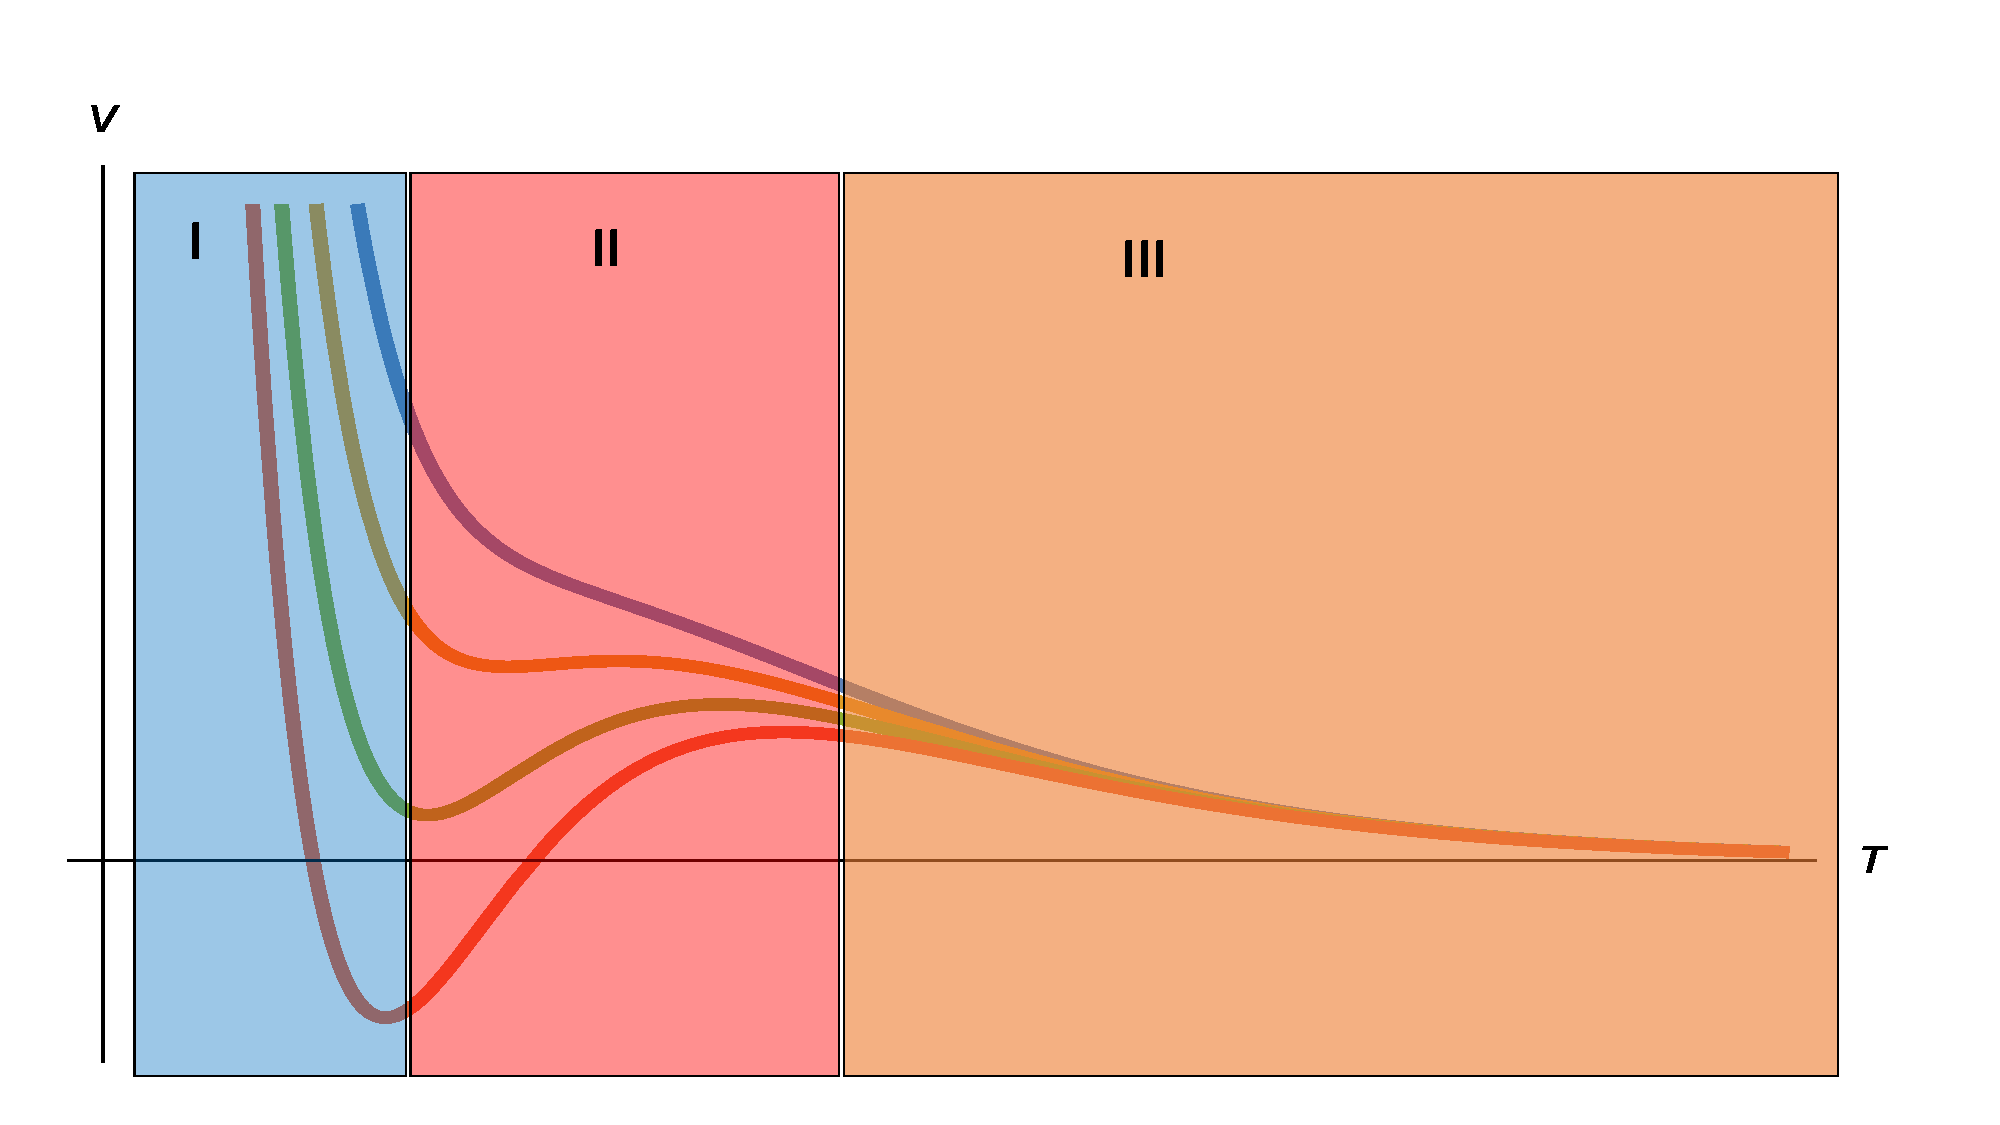
\includegraphics[width=120mm,height=80mm]{Sections/Figures/DineSeiberg.pdf} 
\caption{Dine-Seiberg problem. The scalar potential as a function of the volume or dilaton modulus vanishes asymptotically. Since these fields are the $\alpha'$ and loop expansion parameters respectively, the only region in which these expansions are under full control is the runaway region III. If there is a non trivial minimum it would naturally fall in the small volume/strong coupling region I. In order to obtain reliable minima in the desired region II in which hierarchies  and weak couplings exist (as seen in nature),  compactification parameters, such as integer fluxes or ranks of gauge groups, need to be used.} \label{Fig:CY} 
\end{center}
\end{figure}


\noindent {\it{Constraints from positivity conditions of the stress tensor:}}  Positivity conditions obeyed by stress 
tensors of low energy effective actions lead to interesting constraints on the allowed solution space. As the 10 and 11-dimensional
supergravity theories that arise in string theory obey the strong energy condition, this leads to an important no-go theorem \cite{Gibbons:1984kp, deWit:1986mwo, Maldacena:2000mw}.

The general 10-dimensional metric consistent with maximal symmetry in 4 dimensions is of the form
$$ 
  ds^{2} = g_{MN} dx^{M} dx^{N} = e^{2A(y)} \tilde{g}_{\mu \nu} dx^{\mu} dx^{\nu} + g_{mn}(y) dy^{m} dy^{n},
$$
where $\tilde{g}_{\mu \nu}$ is the metric of a maximally symmetric space in 4 dimensions. The trace reversed Einstein equation in the non-compact directions reads
\begin{equation}
 R_{\mu \nu} = \tilde{R}_{\mu \nu} - \tilde{g}_{\mu \nu} \left( \nabla^{2} A + 2 ( \nabla A)^{2} \right) = T_{\mu \nu} - {1 \over 8} e^{2A} \tilde{g}_{\mu \nu} T^{L}_{\phantom{L} L} \ .
\end{equation}
Contracting this with $g^{\mu \nu}$ one finds
\begin{equation}
\label{gauss}
  \tilde{R} + e^{2A} \hat{T} = 2 e^{-2A} \nabla^{2}  e^{2A},
\end{equation}
where we have defined
\begin{equation}
\label{hatT}
  \hat{T} =  - T^{\mu}_{\phantom{\mu} \mu} + {1 \over 2} T^{L}_{\phantom{L} L}
   = {1 \over 2} \left( - T^{\mu}_{\phantom{\mu} \mu} + {1 \over 2} T^{m}_{\phantom{m} m} \right) \ .
\end{equation}
It is easy to check that $\hat{T}$ is positive semi-definite for all $p$-form flux configurations which are consistent with maximal symmetry. In particular, it is positive semi-definite for $p \geq 1$ and vanishes for $p=1$. Now, multiplying (\ref{gauss}) by $e^{2A}$ and integrating over the compact manifold one concludes that dS compactifications are impossible while Minkowski compactifications allow only 1-form flux. This `no-go theorem' can be evaded by making use of local terms in the supergravity action. For example, orientifold planes in IIB string theory carry negative tension and provide  (localised) negative contributions to $\hat{T}$. Furthermore higher derivative corrections, loop corrections and non-perturbative effects will in general modify (\ref{gauss}). 

The above result has been generalised to various settings in  \cite{Hertzberg:2007wc, Green:2011cn, Gautason:2012tb, Quigley:2015jia, Kutasov:2015eba, Basile:2020mpt, Andriot:2022xjh}.
In particular,  \cite{Kutasov:2015eba} obtained a no-go theorem for dS solutions (of any dimensionality) to all orders in the $\alpha'$ expansion
in heterotic strings  (recently this was generalised to one loop in a specific setting involving string theory without spacetime supersymmetry \cite{Baykara:2022cwj}). Implications for other string theories follow from dualities. 

Attempts to construct dS space in string theory always involve the inclusion of corrections to the effective action which allow for the evasion of the no-go theorems. That said, we note that there also exist arguments that the obstacles to dS are deeper and more fundamental than simply the absence of particular objects in the low-energy supergravity theory. For examples of these principled obstructions to dS, see 
\cite{ Obied:2018sgi, Banks:2012hx, Banks:2019oiz, Brennan:2017rbf, Danielsson:2018ztv}  (the Swampland dS conjectures will be discussed in
Sec. 7) and also \cite{Sethi:2017phn} for an alternative perspective.

We next discuss the generation of moduli potentials -- moduli stabilisation -- in various string theories. Our focus will be on the form of the effective potential and Minkowski/AdS/dS solutions in four dimensions. Time-dependent cosmological solutions will be discussed in the later sections. We start with arguably the most developed constructions, those of type IIB string theory.

\subsection{Moduli Stabilisation: IIB}

\label{sec:dSstrings}

Moduli stabilisation in the context of semi-realistic vacua (i.e.~incorporating hierarchies and supersymmetry breaking) is best understood in the context of type IIB models and we start by discussing these models. In type IIB, for a special (albeit large) choice of the fluxes and localised sources,
one has  the knowledge of 10-dimensional solutions which incorporate the backreaction of fluxes. These fluxes also stabilise the dilaton and complex structure moduli.  This class is often referred to as pseudo-BPS. We discuss these  following \cite{Giddings:2001yu, Dasgupta:1999ss, Gukov:1999ya} (see  e.g.  \cite{hep-th/0012213, Taylor:1999ii, Michelson:1996pn} for earlier work).  The construction of these solutions starts by considering an orientifolded Calabi-Yau (all field configurations and fluctuations are required to be consistent with the orientifolding, for details see \cite{Grimm:2004uq}). The
3-form fluxes of the IIB theory, $F_3$ and $H_3$ are turned on and satisfy Dirac quantisation conditions
\begin{equation}
\setlength\fboxsep{0.25cm}
\setlength\fboxrule{0.4pt}
\boxed{
\label{fluxquanta}
{1 \over 2 \pi \alpha'}  \int_{\Sigma_{3}} F_3 \in 2 \pi \mathbb{Z},  \phantom{abc} {1 \over 2 \pi \alpha'}  \int_{\Sigma_{3}} H_3 \in 2 \pi \mathbb{Z}.
}
\end{equation}
These thread the 3-cycles of the Calabi-Yau. The 10-dimensional Einstein frame metric takes the form
\begin{equation}
\label{gkpxx}
  ds^2 = e^{-2A(y)} \eta_{\mu \nu} dx^{\mu} dx^{\nu} + e^{2A(y)} \tilde{g}_{mn}(y) dy^{m} dy^{n},
\end{equation}
where $\tilde{g}_{mn}(y)$ is the metric of the underlying Calabi-Yau  and $e^{-2A(y)}$ is the `warp factor'. Thus, one is naturally
led to warped compactifications with an internal manifold which is conformal to a (orientifolded) Calabi-Yau -- an appealing aspect since it preserves
much of the structure and intuition of pure CY compactifications.\footnote{The metric does not take the form (\ref{gkpxx}) for general solutions in IIB; this form applies only for those in the pseudo-BPS class. We will describe below the conditions that this implies on the localised sources and fluxes.}

The warp factor is sourced by 3-form flux and localised objects\footnote{These have to be space-filling to maintain Poincare invariance.
} which carry D3-charge and is determined by the equation:
\begin{equation} 
\label{warpf}
\setlength\fboxsep{0.25cm}
\setlength\fboxrule{0.4pt}
\boxed{
 -  \tilde{ \nabla}^{2} e^{-4A} =   { G_{mnp} \tilde{G}^{mnp}  \over {12 {\rm{Re }} S} } + 2 \kappa_{10}^2 T_{3} \tilde{\rho}^{\rm loc}_3
 }
\end{equation}
where $S =  g_s^{-1} - i\,C_0$ is the axio-dilaton, $G_{3} = F_3 - iS H_3$ is the complexified 3-form flux, $\tilde{\rho}^{\rm loc}_{3}$
is the localised $D3$ brane charge density and $T_3$ the tension of D3-branes in the 10-dimensional Einstein frame. The superscript
tilde is used to indicate the use of the metric $\tilde{g}_{mn}$.

The localised sources which contribute to the D3-charge are D3-branes and O3-planes which are point-like in the extra dimensions, as well as D7-branes and O7-planes which wrap four cycles of the Calabi-Yau (these are the only localised sources allowed for these pseudo-BPS solutions).   Note that the contribution of the fluxes to the right hand side of (\ref{warpf}) is positive definite. Thus, cancellation of the $D3$ tadpole condition requires the presence of carriers of negative $D3$ charge. This is provided by the O3-planes\footnote{As mentioned above, the orientifold planes are central to the very existence of these compactifications, as they have a negative tension and hence can provide a negative contribution to $\hat{T}$ (as defined in (\ref{hatT})). This evades the no-go theorem and enables the existence of warped Minkowski compactifications.} or wrapped D7-branes. Thus, the choice of flux quanta is limited to those whose total D3-charge is less in magnitude than the upper bound set by the contributions from the negative charge carriers.\footnote{The solutions can be generalised to F-theory, where, the induced D3-charge from the D7-branes D3 is given by the Euler number of the associated four-fold X, $Q_{\rm D3} = { \chi(X) \over 24}$.} While finite (see for instance \cite{Bakker:2021uqw,Grimm:2021vpn}), the number
of consistent flux configurations for a given Calabi-Yau can be enormous, leading to the idea of the string landscape
\cite{Bousso:2000xa, Feng:2000if,Susskind:2003kw, Denef:2007pq}. We will discuss this in more detail in Sec. \ref{ssec:landscape}.

The equations of motion also require that the complexified 3-form flux is imaginary self-dual, i.e.
\be
   G_{3} = i *_6 G_3 \ .
 \label{isd}
 \ee
In terms of Hodge decomposition, this implies $G_3\in(2,1)\oplus(0,3)$ within the Hodge structure of the Calabi-Yau.  
 
In general, these solutions break supersymmetry. Supersymmetry is preserved if $G_3$ is purely $(2,1)$ (it is the presence of a $(0,3)$ component that breaks supersymmetry). Even if supersymmetry is broken at this level, we note that higher order corrections in the 4-dimensional effective action can then restore supersymmetry, and we will see explicit examples of this later in the section.  
   
For a given choice of flux quanta in  (\ref{fluxquanta}), the imaginary self dual condition can be regarded as an equation for the metric and the dilaton, which fixes the values of the complex structure moduli and the dilaton.\footnote{For early work
 on complex structure moduli stabilisation in specific settings  see \cite{Dasgupta:1999ss, hep-th/0201028, Frey:2002hf, hep-th/0312104, Giryavets:2004zr, Conlon:2004ds}.  More recently, explicit studies of the flux induced potential have been carried out in \cite{Cicoli:2022vny, Coudarchet:2022fcl}.  
 An interesting recent development  is the `tadpole conjecture' (see \cite{Bena:2020xrh, Marchesano:2021gyv, Plauschinn:2021hkp, Grana:2022dfw, Lust:2021xds, Lust:2022mhk, Becker:2022hse}). This suggests a tension between stabilising complex structure moduli at generic points in moduli space and keeping the flux-induced contribution to the D3-tadpole within the bounds allowed by the orientifold.}
As a result of the presence of fluxes, complex structure moduli acquire a mass
$$
m_{{\rm cs}} \sim { \Mp \over {\mathcal{V}}}\,, 
$$
where $\mathcal{V}$ is the Einstein frame volume of the internal manifold measured in string units (our frame conventions throughout this section will be those described below equation (\ref{eq:nsnT1})). In general, there is no reason that a particular flux configuration should lead to the dilaton being 
stabilised at weak coupling. To have control over the  effective field theory, only those flux choices that lead to $g_{s} \ll 1$ are relevant. The K\"ahler moduli remain unfixed at this level.  As we will see, these K\"ahler directions can be stabilised at  large volumes by the inclusion of perturbative (in both $\alpha'$ and $g_s$) and non-perturbative corrections to the effective action.  This leads to isolated vacua at  $g_{s} \ll 1$ and large volume,
 where the effective field theory is under control. For this reason, models combining moduli stabilisation, hierarchies and supersymmetry breaking are best understood in type IIB and several proposals for the construction of dS vacua have been made in the setting. 
 
A further phenomenologically appealing feature of the solutions is the presence of regions in the internal manifold with large warping.  The compactifications therefore provide a realisation of the ideas of Randall and Sundrum \cite{Randall:1999ee, Randall:1999vf} in an ultraviolet complete setting. Large warping arises when fluxes thread a shrinking 3-cycle. For instance, if $M$ units of flux thread the shrinking `A cycle' of a conifold
singularity and $K$ units thread its dual `B cycle', then the conifold singularity is resolved and the warp factor on the minimal volume $S^{3}$ associated with the resolution is
$$
  e^{A_{\rm 0}} =  {\rm{exp}} \left( -2\pi K \big{/} 3 M g_s \right).
$$
Note that this factor is exponentially small in the integer flux quanta.  Locally, the geometry is well described by the Klebanov Strassler solution \cite{Klebanov:2000hb} and such regions of large warping are often referred to as warped throats. Warped throats have a wide variety of phenomenological applications and will appear repeatedly in our discussion of cosmological models.
    
We next turn to the 4-dimensional effective action describing the low energy fluctuations about these backgrounds (obtained once the Kaluza-Klein modes are integrated out). This is crucial for developing K\"ahler moduli stabilisation and also provides a complementary 4-dimensional perspective for looking at the complex structure moduli stabilisation. 
   
 We first describe  basic features of the effective action (see  \cite{Giddings:2001yu,  Grimm:2004uq} for  further details).
The relevant closed string fields are the   complex structure moduli $U_a$, $a=1,\cdots, h_{-}^{1,2}$ (the number of harmonic $(2,1)$-forms of the Calabi-Yau that are odd under the orientifold involution), the  axio-dilaton $S$, and the K\"ahler moduli $T_i$, $i=1,\cdots, h^{1,1}$. For simplicity, here we discuss the case where $h^{1,1}_{-} = 0$ (for a detailed analysis of the effective action for compactifications with $h^{1,1}_{-} \neq 0$ see \cite{Grimm:2004uq}, and e.g.~\cite{Cicoli:2021tzt} for a recent discussion). The K\"ahler moduli are then complexified by the definitions:
$$
\setlength\fboxsep{0.25cm}
\setlength\fboxrule{0.4pt}
\boxed{
    T_{i} = {1 \over 2} \int_{\Sigma_{i}} J \wedge J + i \int_{\Sigma_{i}} C_4 \equiv \tau_i + i \theta_i \ ,
}
$$
where $J$ is the CY K\"ahler form (in the Einstein frame, in units of the string length $\ell_s = 2 \pi \sqrt{\alpha'}$) and $C_4$ the 4-form potential. The integrals are performed over 4-cycles of the orientifolded Calabi-Yau. 

 In the language of $\mathcal{N}=1$ supersymmetry, the fields lie in chiral multiplets and the low energy effective action is specified by the K\"ahler potential and superpotential. The tree-level K\"ahler potential (in the limit of large volume) is given by 
\begin{subequations}
\label{eq:nsnT3}
\begin{empheq}[box=\widefbox]{align}
K&= K_{\rm kah} + K_{\rm dil} + K_{\rm cs} \cr
&= -2\ln\vo-\ln\left(S+\overline{S}\right)-\ln \left(-i\, \int_X \Omega\wedge \overline{\Omega}\right) ,
 \label{Ktree}
 \end{empheq}
\end{subequations}
where $\vo = \ell_s^{-6} \int_X \sqrt{g_{(6)}}\, d^6 y$ is the volume of the internal manifold (in the Einstein frame) in units of the string length $\ell_s$. The internal volume $\vo$ is a homogeneous function of degree $3/2$ of the real parts of the K\"ahler moduli $\tau_i$, the volumes of the four cycles. $\Omega$ is  the holomorphic $(3,0)$-form of the manifold. The effect of fluxes is captured 
by the Gukov-Vafa-Witten superpotential \cite{Gukov:1999ya}:
\be
\setlength\fboxsep{0.25cm}
\setlength\fboxrule{0.4pt}
\boxed{
W_\flux=\int_X G_3\wedge \Omega .
\label{Wflux}
}
\ee

Recall that the F-term supergravity scalar potential for a  superpotential $W(\Phi_I)$ and K\"ahler potential $K(\Phi_I, \overline{\Phi}_{\bar{I}})$ is  given by (in units where $\Mp = 1$):
\be
\setlength\fboxsep{0.25cm}
\setlength\fboxrule{0.4pt}
\boxed{
V_F= e^K\left(K^{I\overline{J}}\, D_{I} W {D}_{\overline{J}} \overline{W} - 3|W|^2\right) \,,
\label{VF}
}
\ee
where $K^{I \overline{J}}$ is the inverse of the K\"ahler metric and $D_{I}$ are  K\"ahler covariant derivatives:
 $D_{I} \equiv  \partial_{I} + (\partial_{I} K) W$. For the K\"ahler potential (\ref{Ktree}) and superpotential (\ref{Wflux}), the 
 potential (\ref{VF}) only depends on the K\"ahler moduli through the overall prefactor $e^K$. This comes from a combination of the following facts:

\begin{itemize}

\item The superpotential (\ref{Wflux}) is independent of the K\"ahler moduli. This is obvious from its expression, as the holomorphic 3-form only depends on the complex structure data. But, there is also a symmetry reason behind this perturbative absence of the K\"ahler moduli from the superpotential. The imaginary part of the 
K\"ahler moduli are axionic fields which enjoy shift symmetries $T_i\rightarrow T_i + i\, c_i$ with constant $c_i$'s. This, together 
with the fact that the superpotential is holomorphic, implies that the superpotential cannot depend on $T_{i}$ (within perturbation theory). This shift symmetry is preserved to all orders in perturbation theory \cite{Burgess:2005jx, Witten:1985bz, Burgess:1985zz, Dine:1986vd}, and hence the superpotential is independent of the K\"ahler moduli to all orders in perturbation theory.

\item The K\"ahler potential is of the no-scale form \cite{Cremmer:1983bf, Ellis:1983sf} i.e $K^{T_i\overline{T}_{\bar{\jmath}}} K_{T_i} K_{\overline{T}_{\bar{\jmath}}}=3$. This is a consequence of the fact that the volume $\mathcal{V}$ is a degree $3/2$ homogeneous polynomial in $\tau_i$.

\end{itemize}
With this, the potential is solely a function of the complex structure moduli and the dilaton:
$$
  V^{\rm no-scale}_{F}  = e^K K^{\alpha\overline{\beta}}\, D_{\alpha} W \overline{D}_{\overline{\beta}} \overline{W},
$$
where the indices $\alpha, \beta$ now run only over the complex structure moduli and the dilaton. The potential is minimised
by solving 
$$D_{\alpha} W = 0.$$
This can be shown to be equivalent to the imaginary self-dual condition on the fluxes (\ref{isd}).
At the minimum, the potential vanishes (consistent with the fact that these are Minkowski compactifications). Since $D_{\alpha} W$ are proportional to the corresponding F-terms, this means that the complex structure and dilaton moduli do not break supersymmetry, however the F-terms
of the K\"ahler moduli ($F_i = D_{T_{i}}W$) are non-vanishing and supersymmetry is broken unless $W=0$ (which is equivalent to $G_{3}$ being $(2,1)$ ).
These reflect the standard properties of no-scale vacua: a vanishing vacuum energy $V=0$ together with broken supersymmetry.

Let us next discuss the stabilisation of the K\"ahler moduli. As discussed above, the shift symmetries of the axionic parts of the K\"ahler moduli forbid their appearance in the superpotential to all orders in perturbation theory. However, as these moduli represent the gauge couplings for matter fields on D7-branes, non-perturbative effects like gaugino condensation on D7-branes or Euclidean D3-instantons can generate a superpotential for them (see  \cite{Blumenhagen:2009qh} for a review). The full superpotential for closed string moduli takes the form:
\be
W=W_{\rm flux}(S,U)+W_{\rm np}(S,U,T)\,.
\label{Wtotal}
\ee
The K\"ahler potential  for the K\"ahler  moduli receives various perturbative corrections. In general,
the no-scale condition $K^{T_i\overline{T}_{\bar{\jmath}}} K_{T_i} K_{\overline{T}_{\bar{\jmath}}}=3$, satisfied by the tree level K\"ahler potential, will be 
broken by these corrections. We denote the corrections by $K_{\rm p}$, i.e. 
\be
\label{kcor}
  K_{\rm kah} =  -2\ln\vo + K_{\rm p}.
 \ee
The correction terms $W_{\rm np}$ and $K_{\rm p}$ in (\ref{Wtotal}) and (\ref{kcor}) lead to a potential for the K\"aher moduli. This potential generates a minimum for the moduli,
stabilising them, and is also crucial for understanding the moduli dynamics in a cosmological context.

There are two major scenarios for fixing the K\"ahler moduli. These are the  KKLT construction \cite{Kachru:2003aw} and the Large Volume Scenario (LVS) \cite{Balasubramanian:2005zx}, which we now describe these in detail. Other proposals for K\"ahler moduli stabilisation within the ambit of IIB flux compactifications include \cite{vonGersdorff:2005bf, Berg:2005yu, Westphal:2006tn, Cicoli:2012fh,Gallego:2017dvd, Antoniadis:2018hqy, AbdusSalam:2020ywo}. The most pertinent details of these two main constructions are   
\begin{itemize}
    
\item The KKLT construction  makes use of the fact that the vacuum expectation value of the flux superpotential can be tuned to small values. 
   This serves as a small parameter, allowing for various contributions to the potential arising from $W_{\rm np}$ to compete. The result is 
   an AdS minimum which is supersymmetric.
   
\item The LVS construction makes use of the perturbative no-scale breaking effect in  (\ref{kcor}) driven by  a $\vo$-dependent $\alpha'$ correction. This competes with a non-perturbative correction on a small (blow-up) 4-cycle, resulting in a non-supersymmetric AdS minimum. At the minimum, the volume $\vo\sim e^{1/g_s}\gg 1$ is exponentially large in string units. Supersymmetry continues to be broken by the F-terms associated with the K\"ahler moduli.
\end{itemize}


\subsubsection{The KKLT construction}

As we have seen, the effect of turning on fluxes in type IIB is to generate a potential for the dilaton and complex structure moduli, while leaving the K\"ahler moduli flat. The first step in the KKLT construction involves integrating out the dilaton and complex structure moduli, and then considering the low energy effective action for the K\"ahler moduli alone.  Although a realistic model will have multiple K\"ahler moduli, we will work with a single modulus to illustrate the basic features of the model. The non-perturbative contribution to the superpotential can arise as a result of Euclidean D3-branes or gaugino condensation on wrapped D7-branes.
In both cases, the  superpotential takes the form\footnote{For a superpotential to be generated, the divisor associated with the Kahler modulus has to be
rigid or be rigidified by the presence of fluxes  see e.g. \cite{Witten:1996bn, Kallosh:2005yu, Kallosh:2005gs, Bianchi:2011qh, Blumenhagen:2009qh, Kim:2022uni,  Alexandrov:2022mmy, Kim:2022jvv, Kim:2023cbh} for technical discussions. Recently, there have been conjectures on challenges in generating such a superpotential term \cite{Lust:2022lfc}. }
$$ 
  W_{\rm np} = A(U, S) \,e^{ -a T},
$$
where the pre-factor $A$ is a function of complex structure moduli $U$ and the dilaton $S$, but has no dependence on the K\"ahler moduli. 
The constant `$a$' is equal to $2 \pi$ when the effect is generated by Euclidean D3-branes, while in the case of gaugino condensation on wrapped D7-branes  $a = 2 \pi \big{/} N$, where $N$ is the rank of the condensing gauge group. With the dilaton and complex structure moduli integrated out, the flux superpotential makes a constant contribution to the superpotential $(W_0)$. The full superpotential is then
$$
W = W_0 + A\,e^{-aT}.
$$
A key requirement of KKLT is that the fluxes are tuned so that $|W_0| \ll 1$. Working with the tree-level K\"ahler potential $K = - 3 \log \left( T + \overline{T} \right)$, the resulting potential is 
$$
 V = { |a A|^{2} \over 6 \tau}  e^{-2a \tau} + {a |A|^2 \over 2 \tau^{2} } e^{-2a\tau} + {{a \,{\rm{Re}}(A W_0^{*} e^{-i \theta})} \over 2 \tau^{2} } e^{-a\tau}.
 $$
After adjusting the phase of the axion to its minimum, one obtains a supersymmetric minimum $D_TW=0$ with 
$$
   \tau \sim { 1\over  a}   \ln  { |W_0|^{-1}  } > 1\,.
$$
From the logarithmic dependence of $\tau$ on $|W_0|$, we understand why a small $|W_0|$ is a key requirement of the construction. The existence of a large number of choices of flux quanta which lead to small values of $|W_0|$ follows from statistical considerations \cite{Denef:2004ze}. Recently, explicit constructions with $|W_0|$ as low as $10^{-120}$ have been carried out  \cite{Demirtas:2019sip,Demirtas:2021nlu} (for earlier work on obtaining 
low values of $|W_0|$ see \cite{Cole:2019enn,Denef:2004dm,hep-th/0312104, Conlon:2004ds}). Sufficiently large $\tau$ is necessary to ensure that any perturbative corrections to the K\"ahler potential yield sub-leading contributions to the
potential that we can safely ignore, and thereby justifying the use of the tree level K\"ahler potential. Furthermore, 
the masses of the K\"ahler moduli are \cite{Choi:2004sx, Choi:2005ge}
$$
  m_{T} \sim m_{3/2} \ln \left( \frac{M_P}{m_{3/2}} \right), 
$$
where the gravitino mass $m_{3/2} = e^{K/2} \vert W \vert$. Although logarithmically enhanced compared to $m_{3/2}$, this implies that the masses of the K\"ahler moduli are parametrically lighter than those of the complex structure moduli, as required for the consistency of
the 2-step procedure. For work on realising  the KKLT construction in explicit settings, see e.g. \cite{Denef:2004dm, Denef:2005mm, Demirtas:2021nlu}.

Note that the no-scale structure present in the pure flux GKP compactifications is absent from KKLT; the process of stabilisation generates a supersymmetric vacuum and returns the mass of the K\"ahler modulus to above that of the gravitino mass. This is an important qualitative difference between KKLT and LVS, which we now discuss, where the no-scale structure survives in the leading approximation.

\subsubsection{The Large Volume Scenario}
 
The starting point for the LVS construction \cite{Balasubramanian:2005zx} is the same as for KKLT, namely the low energy effective field theory after the complex structure and the axio-dilaton have been integrated out. LVS requires at least two moduli, with the Calabi-Yau having some form of `Swiss-cheese' structure, i.e described by an overall volume with subsequent moduli representing geometric `holes' corresponding to blow-up moduli. The simplest realisation is for the case of two K\"ahler moduli. Here the expression for the volume of the Calabi-Yau takes the form:
$$
  \vo=\tau_b^{3/2}-\tau_s^{3/2},
$$
where $\tau_b$ is volume of a big 4-cycle (in Einstein frame) and $\tau_s$ measures the volume of a hole in it (more precisely $\tau_s$ controls the volume of an exceptional del Pezzo divisor resolving a point-like singularity). The leading $\alpha'$ correction to the K\"ahler potential \cite{Becker:2002nn} is included,
 $$
     K = -2\ln\left(\vo+\frac{\xi}{2}\left(\frac{S+\overline{S}}{2}\right)^{3/2}\right),
 $$
with $\xi\equiv -\frac{\chi(X) \zeta(3)}{2(2\pi)^3}$ where $\chi(X)$ is the Euler number of the Calabi-Yau and $\zeta$ is the Riemann zeta function. LVS also requires a non-perturbative effect supported on the small cycle,
\bea
W &=& W_0+A_s\,e^{-a_sT_s}\,.
\eea
As discussed above, here $a_s= 2\pi \big{/} N$ in the case that the effect arises as a result of gaugino condensation and $a_s=2\pi$ in the case of wrapped
Euclidean branes. Working in the limit $\tau_b \gg \tau_s$, after  fixing the axionic partner of $\tau_s$ at its minimum, the scalar potential (\ref{VF}) takes the form:
\be
V =\frac43\frac{a_s^2A_s^2\sqrt{\tau_s}e^{-2a_s\tau_s}}{s\mathcal{V}}-\frac{2a_sA_s|W_0|\tau_s \, e^{-a_s\tau_s}}{s\mathcal{V}^2}+\frac{3\sqrt{s}\,\xi \, |W_0|^2}{8\vo^3}\,.
\label{VLVS}
\ee
Minimising the potential\footnote{Here, s is to be thought of as parameter, it is fixed along with the complex structure moduli as result of the presence of fluxes.}, one finds a minimum at
\be
\langle\vo\rangle \simeq \frac{3\sqrt{\langle\tau_s\rangle}\,|W_0|}{4a_s A_s}\,e^{a_s \langle\tau_s\rangle}\qquad\text{and}\qquad \langle\tau_s\rangle \simeq \frac{1}{g_s}\left(\frac{\xi}{2}\right)^{2/3}\,.
\label{LVSmin}
\ee
Let us stress some important aspects of the scenario:
\ben

\item The minimum arises as a balance between an $\alpha'$ correction (giving a term in the potential scaling as $\vo^{-3}$) and non-perturbative effects on the small 4-cycle (which are definitely generated for a rigid del Pezzo divisor like $\tau_s$). As a result, the overall volume is exponentially large in the size of the small 4-cycle.

\item The construction generalises to the situation with multiple blow-up moduli. In the general situation with blow up and fibre moduli, the fibre moduli can be stabilised by loop effects \cite{Cicoli:2008va} or higher derivative corrections \cite{Cicoli:2016chb}. Moduli stabilisation in the large volume scenario has been extensively studied, see \cite{Conlon:2005ki, Berg:2005yu, Berg:2007wt, Blumenhagen:2007sm, Conlon:2010ji, Cicoli:2011qg, Cicoli:2012vw,  Cicoli:2013mpa,  Cicoli:2013cha, Reece:2015qbf, Cicoli:2016xae, Cicoli:2017shd, Gallego:2017dvd, Cicoli:2017axo} and  \cite{AbdusSalam:2020ywo, Cicoli:2021dhg, Gao:2022fdi, Junghans:2022exo, Leontaris:2022rzj, Junghans:2022kxg} for recent studies.

\item In LVS models, a small value of the dilaton helps guarantee that the effective field theory is under control. For  $g_s\lesssim 0.1$, (\ref{LVSmin}) implies
that $\tau_b$ and $\tau_s$ are much larger than the string scale, and hence the use of the supergravity approximation is justified. 

\item The models can be constructed  for natural values of $|W_0|$; $W_0 \sim \mathcal{O}(1-10)$. See \cite{Cicoli:2013swa} for a discussion and  \cite{Louis:2012nb} for a concrete example. 

\item The LVS vacuum is AdS with the value of the potential at the minimum $V_{\rm LVS}\sim - m_{3/2}^3 \Mp$. It is  non-supersymmetric with the largest F-term given by $F^{T_b} \sim \tau_b \,m_{3/2}$ (inherited from the no-scale structure). Hence the Goldstino is the fermionic partner of $T_b$ in the corresponding $N=1$ chiral multiplet. This is eaten up by the gravitino which develops a non-zero mass.

\een

\subsubsection{Attractive features of IIB models}

Much of our discussion of cosmological models will be set in IIB flux vacua. There are two major reasons for this: first, the low energy effective action is well understood, and second, this low energy effective action has many attractive features from the point of view of phenomenology. Let us list some of these:

\ben

\item \emph{Controlled flux backreaction}:  The  backreaction of the fluxes on the internal geometry is well understood and leads to internal
manifolds which are conformally Calabi-Yau. The understanding of the resulting underlying moduli space is better than in other settings, with the effect of the warp (conformal) factor on the low energy effective action being negligible at large volume. For progress in computing the  form of the K\"ahler potential including the effects of warping see \cite{DeWolfe:2002nn, deAlwis:2003sn, Giddings:2005ff, Frey:2006wv, Burgess:2006mn, Douglas:2007tu, Shiu:2008ry, Douglas:2008jx,Frey:2008xw, Martucci:2014ska}. 


\item \emph{Suppressed scalar potential scale}: IIB offers vacua at large volume, where there exists a clean separation between the string, Kaluza-Klein and moduli mass scales (recall that the Kaluza Klein scale $M_{\rm KK} \propto  \Mp \big{/} \vo^{2/3}$ and  $M_{\rm s} \propto  \Mp \big{/} \vo^{1/2}$). On the other hand, the mass of the complex structure moduli behave as $M_{\rm cs} \propto  \Mp \big{/} \vo$. Thus, at large volume
$$
M_{\rm moduli} \ll M_{\rm KK} \ll M_{\rm s}.
$$
The moduli effective action therefore provides a good description of the low energy dynamics.

\item \emph{Hierarchically suppressed SUSY breaking scale}: Supersymmetry is broken at tree-level by the F-terms of the K\"ahler moduli which are proportional
to the $(0,3)$ component of $G_3$. The gravitino mass is given by  $m_{3/2}= e^{K/2} W_0 \sim {W_0} \big{/} {\vo}$. This is
hierarchically smaller than the Kaluza-Klein scale for both KKLT (where $W_0\ll 1$) and  LVS models (where $\vo \gg 1$). See  \cite{Cicoli:2013swa}  for a detailed discussion.
  
\item \emph{Progress in computing higher order corrections to the effective action}: Since the K\"ahler moduli are flat at tree level, 
 higher order corrections to the effective action become crucial for their stabilisation and cosmological dynamics. There has been a lot of progress in understanding these.
 
 The first computation in this direction was the $\cN=2$ $\mc{O}(\alpha'^3)$ corrections to the K\"ahler potential $K$ \cite{Becker:2002nn}. Additional $\cN=2$ $\mc{O}(g_s^2 \alpha'^2)$ and $\mc{O}(g_s^2 \alpha'^4)$ contributions to $K$ have been obtained  in \cite{Berg:2005ja} and further advanced  in \cite{Berg:2007wt}. In this context, Ref.~\cite{Cicoli:2007xp} showed the existence of an ``extended no-scale structure" which implies that $\mc{O}(g_s^2 \alpha'^2)$ contributions to the scalar potential vanish. Moreover, Ref. \cite{Bonetti:2016dqh} reconsidered $\cN=2$ $\mc{O}(\alpha'^3)$ contributions to the K\"ahler potential incorporating the backreaction of these terms on the  geometry and found that they lead to moduli redefinitions.  Higher derivative $\cN=2$ $\mc{O}(\alpha'^3)$ terms have been computed in \cite{Ciupke:2015msa, Grimm:2017okk}. 

There has also been substantial progress in understanding  $\cN=1$ perturbative effects. Ref.~\cite{Berg:2014ama, Haack:2015pbv,Haack:2018ufg}  obtained  $\cN=1$ string loop corrections to the Einstein-Hilbert term showing that they generate $g_s^2$ corrections to a term involving the CY Euler number (see also \cite{Antoniadis:2018hqy}).  In \cite{Conlon:2009xf,Conlon:2009kt} it was shown that worldsheet 1-loop corrections can also led to field redefinitions of the K\"ahler moduli at 1-loop level. Ref. \cite{Grimm:2013gma} showed that $\cN=1$ $\mc{O}(\alpha'^2)$ corrections to the effective action  lead to moduli redefinitions, while ref. \cite{Minasian:2015bxa} found that $\cN=1$ $\mc{O}(\alpha'^3)$ effects are captured by a shift of the CY Euler number term.   Recently, a systematic treatment of corrections in the F-theory setting has been carried out in \cite{Cicoli:2021rub}.

It is often not necessary to obtain the full functional dependence of these corrections on all moduli. Rather, it is sufficient to determine their dependence on the K\"ahler moduli (which are the light ones).  The functional dependence of string loop corrections to $K$ on the K\"ahler moduli can often  be determined from generalisations of toroidal computations and low-energy arguments \cite{Cicoli:2007xp, Burgess:2010sy}. Another powerful tool is imposing the positivity of the K\"ahler metric \cite{Conlon:2006gv}. Moreover, ref. \cite{Burgess:2020qsc} used the $2$ scaling symmetries of the 10-dimensional action at tree-level to infer the dependence on the overall volume mode and the dilaton of any arbitrary perturbative correction to the effective action. Recently, the one loop correction to the K\"ahler potential has
been related to a supersymmetric index \cite{Kim:2023sfs}.

 \item \emph{Expansion parameters}:  As mentioned in our discussion of the Dine-Seiberg problem, moduli stabilisation corresponds to fixing the values of fields whose VEVs themselves give the expansion parameters of the theories. Furthermore, the asymptotic weakly-coupled 
 regions in field space correspond to runaway potentials. Thus, an interesting question is: how can small expansion parameters arise when moduli are stabilised?
To answer this, let us start by taking the superpotential and K\"ahler  potential to be of the general form in (\ref{Wtotal}) and (\ref{kcor}). We write the F-term potential as
\be
V=V_0 +\delta V\,,
\ee
where $V_0$ is the tree-level potential and $\delta V$ is the correction term in the potential arising as a result of the correction terms in (\ref{Wtotal}) and (\ref{kcor}). Since $V_0$ is independent of the  K\"ahler moduli, the minimum of the potential in the K\"ahler moduli space is determined by $\delta V$. The leading contribution to $\delta V$  takes the form \cite{Conlon:2005ki}:
\be
\delta V\propto e^K\left( W_0^2 \,K_{\rm p} + W_0\, W_{\rm np}\right)\,.
\label{eq:deltaV}
\ee 
The most obvious regime to consider is  where both the tree level contribution to the superpotential dominates over the non-perturbative part ($W_0\gg W_{\rm np}$) and also the perturbative corrections to the K\"ahler potential are much larger than the non-perturbative corrections to the superpotential
($K_{\rm p}\gg W_{\rm np}$). In this regime,  the first term in (\ref{eq:deltaV}) is  the leading order term. It would lift the potential and give  a runaway behaviour (unless terms of different order in the perturbative expansion compete,  but such a competition will always lead to problems with the
perturbative expansion if there is only one expansion parameter \footnote{Recently an exception to this rule was pointed out in \cite{Burgess:2022nbx} in the sense that there exist cases in QFT for which the perturbative expansion can be resummed as in the renormalisation group case, this may allow for a reliable perturbative minimum for $\mathcal V$ as long as the dilaton has been fixed at weak coupling.}). This is the Dine-Seiberg problem \cite{Dine:1985he} for the setting. 

Type IIB flux compactifications  provide at least  two concrete ways to alleviate the problem:

\begin{itemize}[*]

\item[*] In the KKLT construction, the large discrete degeneracy of flux vacua is used to tune $W_0$ to be exponentially small  so that $W_0\sim W_{\rm np}$. As a result,  terms which are of order $W_{\rm np}^2$  are also required to be included in (\ref{eq:deltaV}). The K\"ahler moduli are stabilised due to competition between terms which are of the order  $W_0\, W_{\rm np}$ and $W_{\rm np}^2$. Note that in this regime corrections to the K\"ahler potential can be consistently neglected since their contribution to the scalar potential is sub-leading.

\item[*] LVS models exploit another possibility. Here, the key idea is that  string compactifications can feature more than one expansion parameter (with each corresponding
to the vacuum expectation value of one of the many fields in string theory). The two terms in (\ref{eq:deltaV}) can consistently compete with each other to generate a minimum so long as each arises from a different expansion. In LVS, the first term in (\ref{eq:deltaV}) is part of an expansion in terms of inverse powers of the overall volume of the compactification $(1 \big{/} \vo)$ while the second term is part of an expansion in the size of non-perturbative effects on a small 4-cycle $(e^{-a_s\tau_s})$. These compete to yield a minimum at large volume.

\end{itemize}

\end{enumerate}

\subsubsection{De Sitter in IIB}

The vacua we have discussed so far are AdS. It is possible to obtain dS vacua either by incorporating additional effects which are part of the low energy
 effective action or taking a more general approach to finding minima of the effective action. Below, we describe various proposals for
  constructions of dS vacua\footnote{For recent summaries of the state of the art in dS constructions   and the challenges involved see for example  \cite{Kachru:2018aqn, Cicoli:2018kdo}.} in the IIB setting, illustrating such general constructions in figures \ref{Fig:CY3} and \ref{Fig:dS1}.

\begin{itemize}

\item {\it Anti-branes}: This was proposed as part of the original KKLT construction  \cite{Kachru:2003aw}.  Anti-D3-branes experience
a potential in the imaginary self dual backgrounds of \cite{Giddings:2001yu}. This drives them  to the bottoms of warped throats within the compactification.
An anti-D3-brane at the bottom of a warped throat makes a positive definite contribution to the potential. This is given by
$$
   V_{\overline{\rm D3}} \sim { e^{4A_0} \over {(T+ \overline{T})^2} },
$$
where $e^{A_0}$ is the value of the warp factor at the bottom of the throat. Such a contribution uplifts the KKLT AdS vacuum to a dS one. 
The introduction of an anti-brane takes the configuration away from the pseudo-BPS class, and
various aspects of the effective field theory remain to be understood (see  e.g. \cite{Bena:2018fqc, Dudas:2019pls, Bena:2009xk, Polchinski:2015bea, Kachru:2019dvo, Bento:2021nbb, Moritz:2018ani, Gao:2020xqh, Gautason:2019jwq, Bena:2022ive} and references therein).  Embedding of the system in a supersymmetric effective field theory by making use of the nilpotent field formalism is discussed in \cite{Kallosh:2015nia} and references therein. A recent construction
\cite{Bena:2022cwb}, provides a way to make dS constructions with anti-D3-branes minimalistic (in addition to keeping the effective field theory under control).

\begin{figure}[t]
\begin{center}
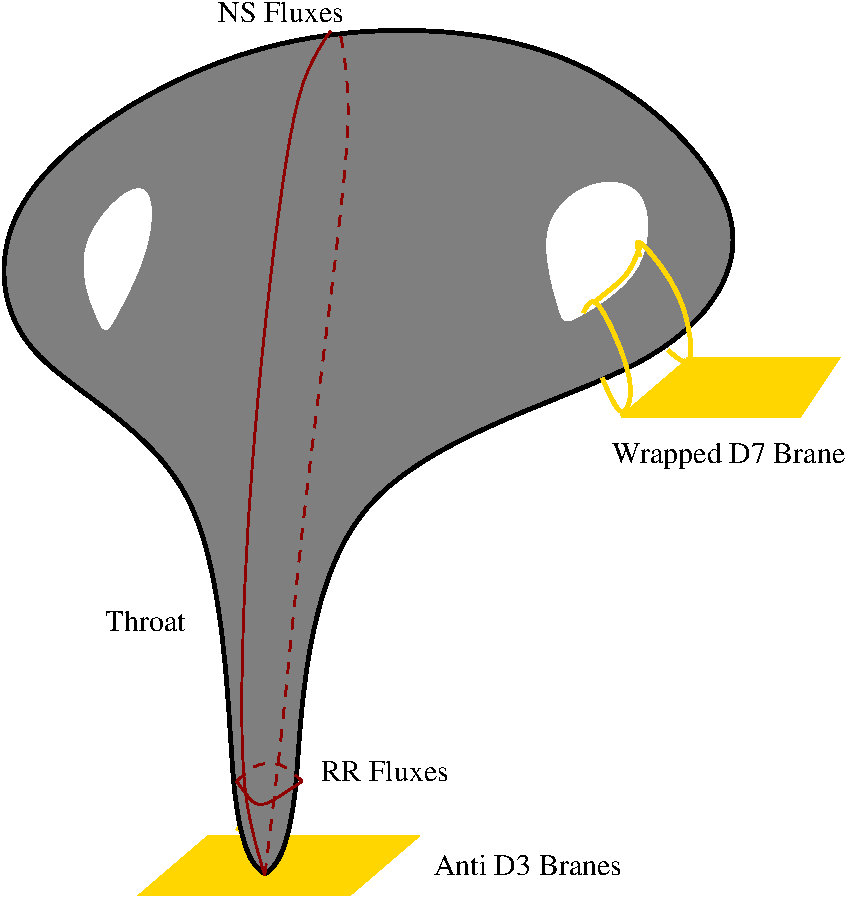
\includegraphics[width=65mm,height=80mm]{Sections/Figures/throatCY.pdf} 
\caption{A cartoon representation of a typical Calabi-Yau configuration as used in KKLT and LVS scenarios. The D7-branes wrapped 4-cycles and may host the gauge theory that provides the corresponding non-perturbative effects in the superpotential. The non-trivial fluxes typically lead to the 3-cycles corresponding to long throats that give rise to warped factors in the metric and may host anti-D3-branes at their tip to provide the dS uplift.} \label{Fig:CY3} 
\end{center}
\end{figure}


\begin{figure}[t]
\begin{center}
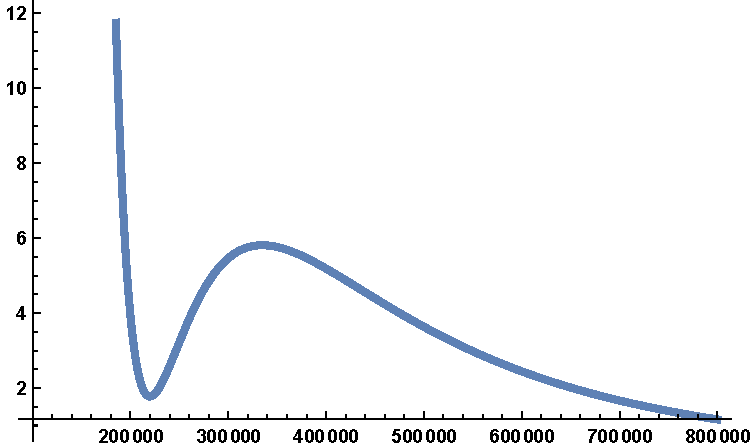
\includegraphics[width=120mm,height=60mm]{Sections/Figures/Potential_dS1.pdf} 
\caption{A typical potential giving rise to dS as illustrated by the minimum at positive value of the scalar potential. The x-axis units represent a cycle volume while the y-axis gives the scalar potential in arbitrary units.} \label{Fig:dS1} 
\end{center}
\end{figure}

\item {\it Magnetised branes} \cite{Burgess:2003ic}: Here, one considers $U(1)$ fluxes localised in a warped throat on D7-branes wrapping the $T$ (volume) modulus. If the vacuum expectation values of the matter fields charged under the $U(1)$ are zero, a term is generated in the effective potential which is exactly of the same form as that arises in the presence of an anti-D3-brane . This term corresponds to a D-term contribution in the 4-dimensional supersymmetric effective action.

\item {\it K\"ahler uplift} \cite{Westphal:2006tn, deAlwis:2011dp, Rummel:2011cd, Louis:2012nb}: The $\alpha'$ corrections to the K\"ahler potential in the KKLT construction can be made to compete with the non-perturbative effects and the flux contributions to produce solutions with positive vacuum energy.  The dS minima so obtained are in regions which correspond to the edge of the validity of the effective field theory. An explicit construction with all geometric moduli stabilised has been carried out in \cite{Louis:2012nb}. 

\item{\it T-branes} \cite{Cicoli:2015ylx}: In the presence of  supersymmetry breaking imaginary self-dual (ISD) 3-form and gauge field fluxes on D7-branes, as in a generic string compactification with orientifolds and wrapped branes, one is led to T-brane configurations. That is, the D7-brane adjoint scalars $\Phi$ are in a configuration for which $\left[ \Phi, \Phi^{\dagger} \right] \neq 0 $. Such configurations provide a positive definite contribution to the 4-dimensional potential which can uplift the AdS minima to dS. Explicit Calabi-Yau orientifold examples with T-brane uplifting in the LVS framework have been derived in \cite{Cicoli:2012vw,Cicoli:2013mpa,Cicoli:2013cha,Cicoli:2017shd,Cicoli:2021dhg}.

\item {\it Dilaton dependent non-perturbative effects} \cite{Cicoli:2012fh}: Here, dilaton-dependent non-perturbative effects coming from E($-1$)-instantons or strong dynamics on  hidden sector of D3-branes at singularities were considered. The non-perturbative term yields a positive definite contribution to the scalar potential similar to that which arises from anti-D3-branes. 

 \item{\it dS vacua from logarithmic/power law loop corrections \cite{Antoniadis:2018hqy, Antoniadis:2019rkh, Berg:2005yu}}: In the presence of 
 intersecting D7-branes,  there are loop corrections
 to the K\"ahler potential whose  contributions to the potential  are logarithmic in the volume of the compatification \cite{Antoniadis:2018hqy, Antoniadis:2019rkh}.  These arise from graviton kinetic terms related to the emission of closed strings on non-vanishing local tadpoles. The logarithmic dependence arises from infrared divergences due to  effective propagation in the two transverse directions to the D7-branes.  
 Combining  the logarithmic terms with  the (usual) power law $\alpha'$ and $g_{s}$ corrections to the potential, one obtains a non-supersymmetric AdS minimum.  dS vacua are obtained by incorporating the  effects of D-term contributions from $U(1)$ magnetic fluxes along the world-volume directions of the D7-branes.  
 
 Closely related are the constructions of \cite{Berg:2005yu}, where it was found that K\"ahler moduli can be stabilised
 by perturbative power law corrections, or those of  \cite{Balasubramanian:2004uy} which used the perturbative $\alpha^{'}$ corrections to generate a dS minimum.
 
 Again, various additional effects can lead to dS minima in the setting. These constructions can provide an avenue to obtain dS vacua without making use of  the non-perturbative part of the superpotential, whose computation involves  various subtleties \cite{Sethi:2017phn}.  

\item {\it Complex structure F-terms} \cite{Gallego:2017dvd}: The potential for the complex structure and dilaton generated by 
fluxes  has  supersymmetric minima where $D_UW_{\rm flux}=0, D_SW_{\rm flux}=0$. There can also be other minima, ones where the F-terms
associated with these fields are non-vanishing. These minima lead to dS vacua once the K\"ahler moduli are stabilised without the need of further ingredients. A concrete example with $\vo\simeq 10^4$ was constructed in \cite{Gallego:2017dvd}.

\item {\it Non-perturbative dS vacua} \cite{Blaback:2013qza}:  Here, dS minima arise from stabilising all the geometric moduli in  one step via the inclusion of  background fluxes and non-perturbative contributions to the superpotential. The key challenge is to develop a good understanding of the $S$ and $U$-moduli dependence of the prefactors of the non-perturbative effects. Duality covariance was used to constrain their form in the analysis. Finding the minima requires sophisticated numerical methods such as genetic algorithms.

\item {\it  Compactifications on Riemann surfaces }\cite{Saltman:2004jh}: This construction makes use of the fact that negative curvature in the 
extra dimensions makes a positive contribution to the 4-dimensional effective potential. In the simplest version, the compactification manifold is a product of 3 Riemann surfaces with one of them having genus greater or equal than 2.
Fluxes are introduced to stabilise the complex structure moduli. At this level, there are  tadpoles for the dilaton and the volumes of each of the surfaces. These are stabilised by the introduction of D7-branes and anti-D7-branes. Supersymmetry is broken at a high scale by the compactification manifold. A related recent development is M-theory on hyperbolic manifolds \cite{DeLuca:2021pej}

\end{itemize}

\subsubsection{Open directions in IIB}

Before moving on to moduli stabilisation in other string theories, we list some interesting open directions in type IIB

\begin{itemize}
\item \textit{Better understanding of higher derivative and $g_s$ corrections}:  Higher derivative
and $g_s$ corrections play a central role in various scenarios for moduli stabilisation. Furthermore, they are important
for checking the validity of the effective field theory used for the construction of the vacua. As we have described above, much progress has
been made in computing these corrections in type IIB. Yet, we still do not have an understanding of all the corrections
in the most general configuration with branes and fluxes. Developing such an understanding is of much 
importance. To give a specific example, it is important to
understand the precise effect  of the logarithmic corrections of  \cite{Antoniadis:2018hqy, Antoniadis:2019rkh} (when they are present; in general, such corrections are absent) in the LVS context, see e.g. \cite{Conlon:2010ji, Junghans:2022exo, Gao:2022fdi}.

\item  \textit{Non-perturbative effects}:  A full understanding of the conditions under which non-perturbative effects in the superpotential are generated  is of importance (see e.g. the discussion in \cite{Sethi:2017phn, Kachru:2018aqn}). Recent progress in this direction includes generalisation of the fermion zero mode conditions  for effective divisors in CY threefolds with singularities along rational curves \cite{Gendler:2022qof}.

\item \textit{The uplift sector}: The introduction of the uplift sector is crucial to obtain dS vacua. This ties the uplift sector
to the  issues  which arise while defining a quantum theory on dS space (see e.g. \cite{Witten:2001kn, Banks:2012hx, Maltz:2016iaw}) and the dS swampland conjecture (see Sec. \ref{Sec:Swamp} for a discussion). Thus, progress in better understanding the physics of the uplift sector  can potentially shed light on various conceptual issues in quantum gravity.

\item  \textit{F-theory moduli stabilisation}: Type IIB models can be thought of as  the weak coupling limit of  F-theory constructions. Thus study of moduli stabilisation in F-theory can potentially lead to novel scenarios and also provide better understanding of existing models. The central issue is  to address moduli stabilisation directly within the F-theory framework. For a review of the phenomenology of F-theory vacua see e.g. \cite{Maharana:2012tu}.

\item \textit{Local curvatures}: Our present understanding   allows for the computation of the volumes of 4-cycles and 2-cycles after moduli stabilisation. This gives information only about the average size of the curvatures; in principle a 2-cycle with volume which is large in string units can be anisotropic and have regions where the curvature is large. While this is a challenge, it is not expected to be a generic issue.
Progress on this front will require explicit knowledge of metrics on Calabi-Yaus, see e.g. \cite{Headrick:2005ch, Ashmore:2021ohf, Gerdes:2022nzr} for work in this direction.

\item \textit{Model scans}: Detailed understanding of models and their phenomenology requires scans over large number of models. To give a specific example, 
the construction of dS vacua requires uplift potentials of very specific magnitude (as an order one increase in the magnitude leads to a runaway). Given this,
isolating concrete models will certainly need an extensive scan over models varying the flux quanta. The large multitude of IIB vacua implies that optimisation strategies are important. Modern computational tools are promising  in this direction (see \cite{He:2017aed, Ruehle:2020jrk, Cole:2021nnt, Abel:2022nje, Abel:2021ddu}).

\item \textit{Open string sector}: Realistic phenomenology requires the introduction of  open string sector(s) which provide the Standard Model degrees of freedom.\footnote{For a recent review on construction of the Standard Model sector in IIB/F-theory see \cite{Marchesano:2022qbx}.} 
Combining stabilisation of the closed and open string modes in a controlled fashion in Calabi-Yaus  is a very demanding task. This is  because of the difficulty to solve the minimisation equations in the presence of a large number of complex structure and open string moduli. Much progress has been made in this direction \cite{Conlon:2008wa,Krippendorf:2010hj, Cicoli:2011qg, Cicoli:2012vw, Cicoli:2013mpa, Cicoli:2013cha, Cicoli:2016xae, Cicoli:2017shd, Cicoli:2017axo} but a globally consistent model with full moduli stabilisation in a controlled dS vacuum is yet be achieved.

\item \textit{The nature of the expansion}: The weak coupling expansion in quantum field theory is an asymptotic expansion. In flux compactifications, the expansion parameters are small but the tadpole constraint implies that one cannot take the limit of arbitrarily small coupling (as is true of asymptotic expansions). It would be interesting to develop the mathematical theory of such expansions and understand them better.
\end{itemize}

\subsection{Moduli Stabilisation: The full diversity of scenarios}

Although type IIB constructions are the most studied, they represent only one corner of string theory. It is therefore necessary to review moduli stabilisation also in other corners of string theory.

\subsubsection{Moduli stabilisation in type IIA}

In type IIB, there are only 3-form fluxes. These only couple to the complex structure moduli, explaining why fluxes in IIB stabilise the complex structure moduli alone.
In contrast, type IIA theory has both the NSNS 3-form and even RR forms in its spectrum. This allows for a rich structure in the
flux superpotential: the 3-form can couple to the holomorphic 3-form  of the compactification manifold (as in the IIB theory), while even RR forms
can couple to the K\"ahler form. Thus one can hope to stabilise all the geometric moduli solely through the presence of fluxes.  Here, 
key challenges are instead the lack of a full understanding of the 10-dimensional solutions incorporating the back reaction of the fluxes and the questions of how to generate hierarchies and supersymmetry breaking. In fact, it is known that the internal manifold can be neither Calabi-Yau nor conformal to a Calabi-Yau once fluxes are turned on. For supersymmetric solutions, the internal manifold has to be half flat with an $SU(3)$ structure \cite{Behrndt:2004mj, Behrndt:2004km,  House:2005yc, Lust:2004ig}.

In view of the difficulty in obtaining 10-dimensional solutions, the approach taken has been to consider configurations which satisfy the tadpole cancellation conditions and compute the energy functional for these. Critical points of this energy functional can be expected to correspond
to solutions to the 10-dimensional equations of motion in the limit of large volume. We will discuss two constructions in more detail. The first will be set in orientifolds of Calabi-Yaus \cite{DeWolfe:2005uu} (see  e.g. \cite{Kachru:2004jr, Derendinger:2004jn,  Aldazabal:2006up, Saueressig:2005es, Villadoro:2005cu, Ihl:2007ah} for related work). The second will involve compactifications on Nil manifolds \cite{Silverstein:2007ac}.

The simplest $\cN = 1$ supersymmetric IIA orientifolds involve an anti-holomorphic involution acting on a Calabi-Yau. The fixed locus of the involution is wrapped by O6-planes. The tadpole cancellation condition for D6-charge takes the form:
$$
    N_{\rm D6}  + \int_{\Sigma} F_0 \wedge H_3 = 2 N_{\rm O6}, 
$$
where $F_0$ is the mass parameter of the IIA theory and $\Sigma$ is a 3-cycle that the 3-form threads. Thus, by a suitable choice of $H_3$ the tadpole can be cancelled without the introduction of D6-branes. The other fluxes can be arbitrary. The effective action for moduli of the orientifold\footnote{
Type IIA orientifolds have $h^{2,1} + h^{1,1}_{-} +1$  scalar moduli, which are part of $\cN=1$ chiral multiplets.} 
in such configurations was computed in \cite{DeWolfe:2005uu} by making use of the formalism of \cite{Grimm:2004ua}. The following interesting features were found:
\begin{itemize}

\item The classical flux potential stabilised all the geometric moduli. The axionic partners of the complex structure moduli remain unfixed. In principle, these can be lifted by Euclidean D2-instantons but, in practice, such massless gravitationally coupled axions are phenomenologically harmless.

\item As opposed to the IIB case, the number of vacua obtained can be infinite.

\item A scaling argument showed that the solutions can be brought to the regime of arbitrarily small values of $g_s$ and arbitrarily 
large volume.\footnote{For an AdS$_3$ solution (for type IIA on $G_2$ orientifolds) with similar features see \cite{Farakos:2020phe}.}

\end{itemize}

 Various open questions remain  in connecting these DGKT configurations to 10-dimensional solutions. The analysis of  \cite{Acharya:2006ne} revealed that the solutions could be lifted to ten dimensions after the O6-plane was smeared. Another issue is the quantum interpretation of the massive IIA theory (see \cite{McOrist:2012yc} for a detailed discussion). Interestingly, no stable dS vacua have been found \cite{Caviezel:2008tf, Flauger:2008ad, Danielsson:2009ff, Caviezel:2009tu, Danielsson:2010bc, Danielsson:2011au, Andriot:2018ept} in the setting. Recently, the AdS vacua have been explored from the holographic perspective  \cite{Conlon:2021cjk, Apers:2022tfm}, revealing an interesting structure including integer conformal dimensions for fields dual to the moduli.
 
The second example we discuss is that of \cite{Silverstein:2007ac}, which is a construction of metastable dS vacua. As in \cite{Saltman:2004jh}, this exploits the fact that negative scalar curvature in the internal dimensions makes a positive contribution to the 4-dimensional scalar potential. The compactification manifold used is a product of 2 Nil 3-manifolds (these have negative scalar curvature). Orientifolds, branes, fractional Chern-Simons forms  and fluxes consistent with tadpole cancellation conditions are considered. With suitable choice of the discrete parameters, the curvature, field strengths, inverse volume, and 4-dimensional string coupling can be made parametrically small, and the dS Hubble scale can be tuned to be parametrically smaller than the moduli masses. However,  various aspects of the effective field theory remain to be explored (see \cite{Haque:2008jz} for a detailed discussion). As the compactification manifold breaks supersymmetry, high scale supersymmetry is a generic prediction of the models. 

\subsubsection{Moduli stabilisation in heterotic strings}

Heterotic string theory was the original set up for model building in string phenomenology, and as such work towards moduli stabilisation also spans across four decades.\footnote{Some early work on cosmological aspects of heterotic string theory can be found in \cite{Kogan:1986tg, Kogan:1986fx, Khlopov:2002gg}.} Nevertheless, although there are by now well-developed landscapes of heterotic Standard Models containing the exact charged spectrum of the MSSM \cite{Lebedev:2006kn, Lebedev:2008un, Anderson:2011ns, Anderson:2012yf, Anderson:2013xka}, it is fair to say that the programme of moduli stabilisation is much less developed.  Moduli stabilisation in heterotic string theories share many ingredients with type II scenarios, but there are also a number of aspects that make the stabilisation of moduli in heterotic string theory more challenging:
\begin{itemize}
\item The matter sector resides in the bulk, rather than localised on D-branes.  This means that the stabilisation of geometric moduli and the dilaton cannot be decoupled from the problem of building a realistic particle physics.  Because the visible sector gauge couplings are set by the 10D dilaton and volume modulus, there are preferred values for the moduli in order to obtain gauge coupling unification at the GUT scale: $g_s^2/\mathcal{V}=\alpha_{GUT}\approx 1/25$ or, equivalently, $\textrm{Re} S \equiv \sqrt{g} e^{-2\phi}=2$, which are at the bounds of validity of the string coupling and weak curvature expansions.  Moreover, the GUT scale is identified with $M_{\rm KK}$, which however is pushed beyond the phenomenological value by the requirement $\mathcal{V} \lesssim 25$ that follows from the previous expressions after imposing $g_s \lesssim 1$.  Indeed, for an isotropic compactification, $M_{\rm KK}\sim M_s/\mathcal{V}^\frac16 \gtrsim 8 \times 10^{16}\,$GeV, where we used $M_s^2 \sim \Mp^2/4\pi \alpha_{\rm GUT}^{-1} \approx (10^{17} \textrm{GeV})^2$, compared with $M_{\rm GUT} \sim 2 \times 10^{16}$GeV.  This can be circumvented by considering anisotropic compactifications e.g. with two large extra dimensions \cite{Hebecker:2004ce, Dundee:2008ts, Buchmuller:2007qf, Loaiza-Brito:2005bto}.

\item The supersymmetry conditions for a Minkowski-CY background, $H = -\frac12 *dJ$, force all the $H$-flux to vanish for a CY (where $dJ=0$) \cite{Strominger:1986uh}, in contrast to type IIB where a supersymmetric background can be obtained for primitive (2,1)-type 3-form flux backgrounds.  Therefore, at leading order, if fluxes are used to stabilise the complex structure moduli in heterotic string theory, one has to pay either by breaking supersymmetry or deforming away from a CY.

\item The only flux available is that from the single NS-NS 3-form $H$.  The flux superpotential is therefore independent of the dilaton; this implies ($i$) flux backgrounds do not have the no-scale cancellation seen in type IIB ($ii$) the dilaton cannot be stabilised by flux alone and non-perturbative effects such as gaugino condensation have to be relied upon.  As will be discussed further below, there is in fact an interesting interplay between $H$-flux and gaugino condensation \cite{Dine:1985rz, Derendinger:1985kk}, due to the perfect square structure in the heterotic effective supergravity theory, which is given in the Einstein frame by:
\begin{equation}
S_{\rm het} \supset \frac{1}{2\alpha'^4}\int d^{10}x\sqrt{-g}\left(-\frac{1}{12}e^{-\phi}\left(H_{MNP}-\frac{\alpha'}{16}e^{\phi/2}\,\overline{\lambda_{10}}\,\Gamma_{MNP}\lambda_{10} \right)^2\right)\,. 
\label{E:perfectsquare}
\end{equation}

\item The $H$-flux is real.  Having only half as many fluxes per modulus compared with type IIB means that one cannot use the discretuum of fluxes to tune the VEV of the flux superpotential to small values \cite{Curio:2005ew} (the existence of a metastable solution to the $2h_{1,2}$ real coupled, partial non-linear differential equations to stabilise the $2h_{1,2}$ real moduli at weak coupling, with $2h_{1,2}$ real flux parameters, leaves little room to further tune $W$ \cite{Cicoli:2014sva}; see also \cite{Anderson:2011cza} for a proof of this in the large complex structure limit); this is dangerous as a large flux superpotential induces large runaways in the K\"ahler moduli and dilaton directions, which is difficult to counterbalance with exponentially suppressed non-perturbative contributions as done in KKLT.  
\item As will be discussed below, small flux superpotentials can be obtained by considering fractional Chern-Simons contributions to $H$.  Indeed, in the heterotic string, perturbative anomalies in spacetime or on the worldsheet imply that the gauge-invariant $H$ takes the form \cite{Rohm:1985jv}:
\begin{equation}
H = dB -\frac{\alpha'}{4}\Omega_3(A)-\frac{\alpha'}{4}\Omega_3(\omega)\,, \label{E:HwithCS}
\end{equation}
with the Chern-Simons invariant $\Omega_3(A)= \textrm{tr}(A\wedge dA)+\frac23 A \wedge A \wedge A$ and similarly for $\Omega_3(\omega)$.  Note that the Kalb-Ramond and Yang-Mills Chern-Simons contributions are leading order in the derivative expansion, whereas the Lorentz Chern-Simons term is higher order.  Whilst the flat bundles from Wilson lines contribute $H$-flux at leading order, anomaly cancellation and the Bianchi identity force the Chern-Simons $H$-flux from a non-standard embedding of the gauge connection into the spin connection to appear at higher order; the latter's contribution to the superpotential in the low energy effective field theory for massless modes must thus be vanishing due to the non-renormalisation theorems \cite{Dine:1986vd}, although -- as we will see -- it can still contribute to the stabilisation of would-be moduli once these are integrated in.
\item In analogy to the open string moduli in type II theories, heterotic string theories have, on top of the geometric moduli and the dilaton, a number of vector bundle moduli.  The moduli space of complex structure and vector bundle moduli does not take the form of a direct product, rather there is some non-trivial mixing imposed by the Hermitian Yang-Mills equations \cite{Witten:1985bz, Anderson:2010mh, Anderson:2011cza, Anderson:2011ty}.  Although in a supersymmetric Minkowski-CY background the complex structure moduli cannot be stabilised by $H$-flux, they may be stabilised by the gauge bundle moduli. This will be discussed further below.
\end{itemize}

We  now review the main moduli stabilisation scenarios for heterotic string compactifications.

\begin{itemize}
 \item \emph{Heterotic orbifold compactifications.}  The MSSM has been successfully constructed in heterotic toroidal orbifold compactifications \cite{Buchmuller:2006ik, Lebedev:2006kn,Lebedev:2008un}.  The 4-dimensional $N=1$ effective supergravity theory describing these models can be derived using a combination of dimensional reduction, conformal field theory \cite{Hamidi:1986vh, Dixon:1986qv, Dixon:1989fj} and target space modular invariance that descends from the underlying torus (the latter is typically broken to some subgroup by Wilson lines) \cite{Ferrara:1989bc, Lauer:1989ax, Ibanez:1992hc}.  Although the dilaton, K\"ahler and complex structure moduli are flat directions at tree-level, non-perturbative effects tend to lift them all.  As the dilaton describes the tree level gauge couplings, it is lifted by gaugino condensation in a non-Abelian hidden gauge sector \cite{Nilles:1982ik, Ferrara:1982qs, Dine:1985rz}.  Moreover, the gauge couplings also receive threshold corrections from massive string states, which depend on several of the K\"aher moduli and all of the complex structure moduli; these are then also lifted by gaugino condensation \cite{deCarlos:1991gq, deCarlos:1992kox} (interestingly, in some cases, target space modular invariance implies that the resulting scalar potential goes to plus infinity in both the small and large modulus limits, ensuring the existence of a metastable minimum somewhere in-between along this direction and hence forcing compactification \cite{Font:1990nt, Cvetic:1991qm, Bailin:1993fm}).  Finally, worldsheet instantons described by metastable untwisted strings formed by twisted strings distributed at distant fixed points, lift all the remaining K\"ahler moduli, which describe the fixed points' separation \cite{Lust:1991yi}.  
 
 These ingredients were combined in \cite{Parameswaran:2010ec}, which studied the moduli stabilisation of all bulk moduli in top-down explicit MSSM models, with 10 real moduli.  With moduli stabilisation being induced entirely non-perturbatively, it may seem reasonable to expect that a small cosmological constant could be achieved; on the other hand, with 10 real moduli directions, a random search for a metastable minimum would only find 1 in every $2^{10}$ solutions.  In fact, although many consistent dS critical points were found (and no AdS ones), they all had large vacuum energies and tachyonic instabilities.  Aside from the search of metastable dS vacua -- or an understanding as to why they do not exist (see \cite{Olguin-Trejo:2018zun, Gonzalo:2018guu, Leedom:2022zdm} for some discussion on implications of modular invariance for the dS swampland proposal) -- there are a number of details which require further attention.  Not all the moduli dependent terms in the $\cN=1$ Lagrangian are computable with current knowledge.  The same goes for the input parameters in the 4-dimensional scalar potential, which are certain (non-Abelian) singlet matter VEVs, $A_\alpha$, that ($i$) `turn on' the worldsheet instanton contributions as $W_{yuk} \sim h_{\alpha\beta\gamma}(T_i) A_\alpha A_\beta A_\gamma$ and ($ii$) give masses via higher order Yukawa couplings to charged hidden matter, which would otherwise prevent gaugini from condensing.  Another important issue is the stabilisation of twisted moduli or `blow-up' modes.
 
 
 \item \emph{Smooth Calabi-Yau compactifications without fluxes.} Heterotic Standard Models have also been successfully built using smooth CY compactifications and algebraic-geometric techniques \cite{Braun:2005ux, Bouchard:2005ag, Braun:2005nv, Anderson:2011ns, Anderson:2012yf, Anderson:2013xka}.  Key ingredients in these constructions are the non-standard embedding of the gauge bundle into the tangent bundle, together with Wilson lines.  It may be possible that these very same ingredients help with the moduli stabilisation, without the need for the fluxes essential in type II.  Indeed, as mentioned above, the number of gauge bundle moduli depends on the values of the complex structure and, viceversa, the number of complex structure moduli depends on the values of the gauge bundle moduli \cite{Witten:1985bz, Anderson:2010mh, Anderson:2011cza, Anderson:2011ty}. The choice of gauge bundle may then be such that all the complex structure moduli and a large number of other moduli are stabilised \emph{at tree level}; in the most restrictive case only one combination of the K\"ahler moduli and dilaton is left as a flat direction in an ${\cal N}=1$ Minkowski vacuum \cite{Anderson:2011cza}.  

 In a bit more detail \cite{Anderson:2010mh, Anderson:2011cza, Anderson:2011ty}, the $\cN=1$ supersymmetry conditions impose that the gauge fields must obey the Hermitian Yang-Mills equations of zero slope: $F_{ij} = 0 = F_{\bar{\imath}\bar{\jmath}}$ and $g^{i\bar{\jmath}}F_{i\bar{\jmath}}=0$.  These conditions become, respectively, F-term and D-term conditions associated with a 4D $\cN=1$ effective scalar potential, which descends from the term in the 10D action: $-\frac{1}{2\kappa_{10}^2}\alpha'\int d^{10}x \sqrt{-g} \left(-\frac12 \textrm{tr}(g^{i\bar{\jmath}}F_{i\bar{\jmath}})^2+\textrm{tr}(g^{i\bar{\imath}} g^{j\bar{\jmath}} F_{ij} F_{\bar{\imath}\bar{\jmath}})\right)$.  For a given choice of vector bundle moduli, the F-term condition that the vector bundle be holomorphic with respect to a given complex structure fixes some -- possibly all -- complex structure moduli. The D-term condition corresponds to the vector bundle being poly-stable with vanishing slope, and it evidently depends on the K\"ahler moduli via the metric components $g^{i\bar{\jmath}}$.  In fact, it also carries a dilaton dependence via one-loop corrections in the weakly coupled string.  Thus the D-term condition fixes some -- possibly all -- K\"ahler moduli and dilaton, with the exception of the overall volume modulus.  In fact, if the mass scale of these stabilised moduli is of the same order as the KK scale, they should not be considered as moduli at all; so the number of moduli in such a compactification is less than that derived from the CY Hodge numbers.  The vector bundle moduli themselves could be stabilised by the non-perturbative effects, where the Pfaffian prefactors in the superpotential are polynomials in the bundle moduli \cite{Buchbinder:2002ic, Buchbinder:2002pr}.

 Ref. \cite{Anderson:2011cza} proved a no-go theorem that a single surviving flat direction could be stabilised by non-perturbative effects, due to the constraints imposed by the U(1) symmetries associated with the D-term stabilisation.  However, if two flat directions survive, they could be stabilised non-perturbatively by gaugino condensation and/or instantons; as this starts from a genuine $\cN=1$ Minkowski vacuum, these non-perturbative effects do not suffer the usual subtleties associated with rolling solutions \cite{Sethi:2017phn}.  See also \cite{Becker:2004gw, Braun:2006th} for related work in the context of heterotic M-theory.  It remains an open question whether or not explicit realisations of this attractive scenario can be realised.

 \item \emph{Heterotic flux compactifications on non-K\"ahler manifolds.}  As noted above, the introduction of $H$-flux in leading order heterotic compactifications deforms away from $\cN=1$ supersymmetric Calabi-Yaus, either by breaking supersymmetry or by leading to a non-K\"ahler internal space \cite{Strominger:1986uh}.  Indeed, the supersymmetry condition $H=-\frac12*\textrm{d}J$, implies that -- for supersymmetric backgrounds -- flux induces non-K\"ahlerity and can only be (2,1) and (1,2).  Going beyond CY manifolds to manifolds with $SU(3)$ structure (a manifold with $SU(3)$ structure is one that admits a globally defined spinor, and thus preserves some supersymmetry) leads one to consider `geometric fluxes' or `torsion', which have even degree and thus the potential to stabilise the K\"ahler moduli at leading order \cite{Strominger:1986uh, LopesCardoso:2002vpf, Becker:2003sh, Becker:2003yv, Gauntlett:2003cy}.  Manifolds with $SU(3)$ structure are characterised in terms of 5 so-called torsion classes $\mathcal{W}_i$ ($i=1,\dots,5$), with $dJ \in \mathcal{W}_1 \oplus \mathcal{W}_3 \oplus \mathcal{W}_4$ and  $d\Omega \in \mathcal{W}_1 \oplus \mathcal{W}_2 \oplus \mathcal{W}_5$  (see \cite{Grana:2005jc} for a review).  The moduli space of general $SU(3)$ structure manifolds is not so well understood.  The simplest non-CY $SU(3)$ structure manifolds are nearly K\"ahler manifolds, which have only the first torsion class $\mathcal{W}_1$ non-vanishing.
 
  Half-flat manifolds arise as the type II mirrors of Calabi-Yaus with NSNS flux \cite{Gurrieri:2004dt}; they have vanishing $\mathcal{W}_1^-$, $\mathcal{W}_2^-$ (imaginary parts of $\mathcal{W}_1$ and $\mathcal{W}_2$), $\mathcal{W}_4$ and $\mathcal{W}_5$ and their moduli space of metrics is identical to that of the mirror Calabi-Yau.  In \cite{Gurrieri:2004dt, Gurrieri:2007jg} it was shown that dimensional reduction of the heterotic string theory on half-flat mirror manifolds, in the large complex structure limit, yields a 4-dimensional $\cN=1$ supergravity whose K\"ahler potential is identical to the mirror Calabi-Yau and whose superpotential is a generalisation  of the well-known Gukov-Vafa-Witten expression, $W \sim \int \Omega \wedge (H+idJ) \sim e_i T^i + \epsilon_a Z^a + \mu^a \mathcal{G}_a$, with, respectively, geometric, NSNS electric and NSNS magnetic flux parameters $e_i, \epsilon_a$ and $\mu^a$; thus we see that all the geometric moduli can be stabilised in these backgrounds.  This result is expected to extend to all $SU(3)$ structure manifolds (see also \cite{LopesCardoso:2003dvb, Becker:2003sh}).  Progress in constructing gauge bundles for $SU(3)$ structure manifolds has been made for the case of nearly K\"ahler manifolds given as group or group coset manifolds \cite{Chatzistavrakidis:2009mh, Lechtenfeld:2010dr, Klaput:2011mz}; backreaction of the gauge fields induced by the Bianchi identity at order $\alpha'$ can further help with the moduli stabilisation \cite{Klaput:2012vv}.  Due to the runaway dilaton, compactifications on nearly K\"ahler or half-flat manifolds yield domain wall solutions at leading order \cite{Lukas:2010mf, Klaput:2011mz}; a maximally symmetric vacuum could be found by introducing other effects, such as gaugino condensation \cite{Klaput:2012vv}.  However, as mentioned, it would be difficult to balance the tree-level $H$-flux against non-perturbative effects that are exponentially suppressed at weak coupling. 
 
 \item \emph{Heterotic flux compactifications with Chern-Simons terms.}
$H$-flux appears in the 10-dimensional supergravity action in a perfect square together with the gaugino fermion bilinear (\ref{E:perfectsquare}).  The supersymmetry conditions on a CY background require this bilinear to vanish \cite{Dine:1986vd, LopesCardoso:2003sp, Frey:2005zz} but by breaking supersymmetry spontaneously, a background $H$-flux and gaugino condensate are compatible with a Minkowski $\times$ CY compactification, with complex structure and dilaton stabilised \cite{Rohm:1985jv}.   Working out how these effects, understood within the 4D effective field theory, are captured by the 10D supergravity theory, has not yet been fully achieved \cite{LopesCardoso:2003sp, Frey:2005zz}.  Note that satisfying the Minkowski condition would require balancing the background $H$-flux against non-perturbative effects that are exponentially suppressed at weak coupling; as discussed above, this cannot be obtained with integer quantised $H$-flux.  Ref. \cite{Gukov:2003cy} therefore considered the $H$-flux sourced by background discrete Wilson lines, via their contributions to the Chern-Simons term in $H$ (\ref{E:HwithCS}); this $H$-flux can be fractionally quantised instead of integer valued (see Ref. \cite{Apruzzi:2014dza} for the computation of Chern-Simons invariants from Wilson line backgrounds, and Ref. \cite{Anderson:2020ebu} for the same from non-standard embeddings).  Vector bundle and K\"ahler moduli could also be stabilised into a supersymmetric AdS solution once threshold corrections are taken into account.  These latter solutions involve some subtleties as they pass through a strong coupling singularity \cite{Gukov:2003cy}, which can be avoided by considering instead worldsheet instantons \cite{Curio:2005ew}.  
 
 \item \emph{Heterotic Large Volume Scenario.} Ref.~\cite{Cicoli:2013rwa} put several of the ingredients previously discussed -- fractional Chern-Simons fluxes, the requirement of a holomorphic slope-stable gauge bundle, tree-level and non-perturbative (including one-loop threshold corrections) superpotentials -- together with $\alpha'$ corrections to the K\"ahler potential, to compose a heterotic version of the Large Volume Scenario.  In this scenario, the complex structure and gauge bundle moduli are stabilised supersymmetrically at leading order, the dilaton non-perturbatively by gaugino condensation and/or worldsheet instantons, and the K\"ahler moduli by subleading perturbative corrections, ultimately breaking supersymmetry spontaneously in a Minkowski or dS vacuum.  If the complex structure moduli are stabilised by fractional flux, then $|W| \sim \mathcal{O}(0.1-0.01)$ and the supersymmetry breaking is high-scale with $m_{3/2} \sim M_{\rm GUT}$; if they are instead stabilised by the gauge bundle, then $|W|$ can be exponentially suppressed and the supersymmetry breaking scale can be low.  It would be important to work out if these scenarios can be realised in a controlled way with explicit top-down constructions.


 


\end{itemize}
 
\subsubsection{Moduli stabilisation in type I}

Moduli stabilisation in type I has been developed in \cite{Antoniadis:2004pp, Antoniadis:2005nu, Antoniadis:2006eu, Kumar:2006er, Antoniadis:2007jq, Antoniadis:2009bg}. So far, the studies have been mostly in a toroidal setting ($T^{6} \big{/} Z_2$ backgrounds).
 Magnetic fluxes  are introduced  on D9-branes that wrap the internal manifold. The boundary term in the open string action 
plays a  crucial role. This modifies the open string Hamiltonian and its spectrum, and leads to constraints on the closed string background fields due to their couplings to the open string action.  The supersymmetry conditions, together with conditions which define a meaningful world-volume theory, put restrictions on the values of the moduli and fix them.  The presence of branes and magnetic fluxes reduces  the $\cN=4$ theory to  an $\cN = 1$ supersymmetric one.

 The simplest version of the model involves an O9-plane and several stacks of D9-branes. Some of the key features are:
 \begin{itemize}
 
 \item   The introduction of oblique (non-commuting) magnetic fields. These are necessary to fix the off-diagonal components of the metric.
 
 \item  The non-linear part of the Dirac-Born-Infeld (DBI) action is used to fix the overall volume.
 
 \item The large radius limit can be attained by appropriate choice of the magnetic flux quanta.
  
 \item The magnetised  branes  lead to D5-brane charge, for which the associated tadpole has to be cancelled (this can be done without
 the introduction of D5- and O5-planes).
  \end{itemize}

  At this level, the axio-dilaton remains unfixed.   It can be fixed by turning on NSNS and RR fluxes. The choice of fluxes can be made so that the background continues to preserve $\cN=1$ supersymmetry and remain in the weakly coupled regime $(g_s \ll 1)$. 

Interesting open directions for type I strings are:
\begin{itemize}

\item Study of the analogous non-supersymmetric backgrounds.

\item Developing a complete understanding of open string moduli stabilisation in the setting.

\item To see if dS vacua can be obtained. For this, understanding various higher order corrections to the effective action are important. One advantage is that a full string theory description is available and this can be used to compute the relevant corrections. The methods developed in  \cite{Bianchi:2007fx} can be useful to compute non-perturbative effects.

\item Implementing the analogous mechanisms in CY compactifications.

\item Counting the number of such vacua and developing an understanding of their statistical properties.
\end{itemize}

\subsubsection {Moduli stabilisation in M-theory} 

M-theory compactifications on manifolds of G2 holonomy lead to 4-dimensional theories with $N=1$ supersymmetry. Phenomenologically viable compactifications with non-Abelian gauge symmetries and chiral fermions arise if the  G2 manifolds have specific types of singularities. Non-Abelian gauge fields are localized on 3-dimensional submanifolds inside the internal space \cite{Acharya:1998pm}. Chiral fermions are supported at points in the internal manifold where there are conical singularities of a particular type \cite{Acharya:2001gy}.  Although many examples of smooth G2 manifolds have been constructed \cite{Kovalev:2001zr, Joyce:2002eb}, an explicit construction of compact G2 manifolds with the singularities required  has not been carried out so far. But such singular manifolds are believed to exist based on dualities between M-theory and  heterotic and type IIA compactifications. The phenomenological studies of these involve assuming the existence of the singularities and exploring the implications.

Upon reduction to 4 dimensions, geometric moduli corresponding to volumes of 3-cycles, $s_i$, pair up  with axionic fields that arise from the dimensional reduction of the $C_3$ potential to yield complex scalars  which are part of $\cN=1$ chiral multiplets. Let us summarise some of the key features of the 4-dimensional effective action that describes moduli dynamics (see e.g. \cite{Friedmann:2002ty} for further details). The K\"ahler potential is
$$
    K =  -3 \ln V_7,
$$
where $V_7$ is the volume of the 7-manifold (in units of the eleven-dimensional Planck length). The volume is known to be a degree $7/3$ homogeneous polynomial in $s_i$, the 3-cycle volumes. We will focus on scenarios in which the moduli are stabilised as a result of condensation in gauge theories which are localised on three-dimensional submanifolds.\footnote{For constructions involving non-trivial background $C_3$ flux see e.g. \cite{Acharya:2002kv,  deCarlos:2004ses, House:2004pm}} For an $SU(N)$ gauge theory, this leads to a superpotential 
\begin{equation}
\label{Mhidden}
   W =  A\, {\rm{exp}} \left( {-2 \pi f_{h} \over N} \right),
\end{equation}
where $f_{h}$ is the hidden sector gauge kinetic function and $A$ is related to the cutoff of the supersymmetric gauge theory. The gauge kinetic functions are related to the moduli fields by relations of the form $f_{h} = N^{i} \phi_i$; where $\phi_i$ are the moduli (in conventions in which the imaginary parts correspond to the volumes of 3-cycles and the real parts are axionic) and $N^{i}$ are integers. The sum runs over all moduli. In general, there are multiple hidden sectors; the superpotential is the sum of contributions of the type (\ref{Mhidden}) arising from each one of them. This leads to a moduli
potential which stabilises all of them. In fact, all the moduli can be stabilised by considering superpotentials that arise from two hidden
sector contributions \cite{Acharya:2006ia, Acharya:2007rc, Acharya:2011kz}. The vacua obtained are AdS. The value of the cosmological constant can be tuned by varying the ranks of the condensing gauge groups. As there are no fluxes, the landscape of vacua is scanned  by scanning through
these ranks. 

Candidate dS vacua have been constructed in  \cite{Acharya:2007rc, Acharya:2008hi}. This was done by including matter fields charged under the hidden sector gauge symmetries.   The dominant contribution to the vacuum energy then arises  from  F -term contributions of  hidden matter fields and there are solutions with a positive value for the cosmological constant. See \cite{Acharya:2012tw} for  a detailed review of these models. 
 
    The most important open direction is to develop an understanding of the  nature of the singularities that can arise in compact  G2 manifolds. With this,
  one can carry out a systematic derivation of the matter content and the associated effective field theory.
  
	
 \subsection{Holographic Approaches to Moduli Stabilisation}
 
The standard approach to moduli stabilisation, as just described in this section, operates through the language and techniques of
effective field theory. It starts with a 10-dimensional quantum string theory. Using dimensional reduction and effective field theory, it aims to describe the dynamics of this theory in a 4-dimensional language in which the string and Kaluza-Klein modes have been integrated out. Vacua of
 this 4-dimensional theory are found and then claimed to be also vacua of the full 10-dimensional theory. This claim is justified
 by computing corrections to the 4-dimensional theory, in both the $\alpha'$ and $g_s$ expansion, and showing that they are small. The smaller we these corrections are computed to be, the better we think we control the vacuum.

Recently, a complementary approach to thinking about moduli-stabilised vacua has appeared. Most scenarios of moduli stabilisation give, at least initially, AdS vacua and additional ingredients are necessary to uplift these vacua to dS solution. We know from the AdS/CFT correspondence that AdS vacua often have an interpretation in terms of dual conformal field theories. Even without an explicit construction of a dual CFT, the symmetries of AdS map onto the symmetries of CFTs \cite{Heemskerk:2009pn}. It is therefore interesting to re-express the properties 
of phenomenologically appealing moduli-stabilised AdS vacua in terms of CFT quantities.

States in the AdS theory correspond to operators in the CFT. Single-particle excitations in the AdS theory correspond to single-trace primary operators in the CFT, while interactions map onto higher-point correlators in the CFT. Although the whole AdS theory can be mapped into the CFT, the simplest relation concerns masses and conformal dimensions,
\be
\setlength\fboxsep{0.25cm}
\setlength\fboxrule{0.4pt}
\boxed{
\Delta_{\Phi} (\Delta_{\Phi} - d) = m_{\Phi}^2 R_{AdS}^2,
}
\ee
where $\Phi$ denotes both a field in $AdS_{d+1}$ and its corresponding dual operator in $CFT_{d}$, $\Delta$ is the conformal dimension and $R_{AdS}$ is the AdS radius. 


The aims of this program are
\begin{itemize}
\item
By rewriting the vacua of moduli-stabilisation scenarios in an alternative language, search for hidden structures that may be opaque when written in the more conventional language of supergravity and dimensional reduction. From the perspective, AdS moduli-stabilised vacua at many different scales appear very similar from a CFT perspective (e.g. \cite{Conlon:2018vov, Conlon:2020wmc} ). Another example of this is the discovery that the mass spectrum of moduli in type IIA DGKT vacua all correspond to integer conformal dimensions in any dual CFT. This is a striking feature whose origin is not yet understood \cite{Conlon:2021cjk, Apers:2022tfm, Apers:2022zjx, Quirant:2022fpn, QuirantPellin:2022vyp, Plauschinn:2022ztd, Apers:2022vfp}.

\item
In the study of CFTs, the bootstrap program has been able to develop some sharp bounds on allowed consistent regimes for CFTs for quantities such as operator dimensions, both ruling out certain possible ranges and isolating some allowed islands which contain consistent theories (see e.g \cite{Simmons-Duffin:2016gjk}). By writing moduli-stabilising scenarios in CFT language, this provides a chance of ruling out particular scenarios (in the case that they could be proved inconsistent through CFT techniques) or giving strong evidence for their consistency (if they were found to exist in an allowed island).

\item Certain swampland criteria applicable to AdS theories may be given a sharper understanding when viewed holographically from the perspective of a dual CFT. Examples include the weak gravity conjecture \cite{Montero:2018fns, Furuuchi:2017upe, Harlow:2018tng, Andriolo:2020lul, Aharony:2021mpc, Palti:2022unw}, and the Swampland Distance Conjecture \cite{Baume:2020dqd, Perlmutter:2020buo}.

\item
The use of CFT techniques may eventually allow an end-run around the need to use perturbative effective field theory arguments to argue for the consistency of such vacua. This would be appealing as, in practice, it is unlikely that all $\alpha'$ or $g_s$ corrections could ever be computed for realistic string vacua with $N=0$ supersymmetry.

\item
Moduli-stabilised vacua exhibiting hierarchies have some unusual features from a CFT perspective. The presence of a small vacuum energy implies the central charge of the CFT is parametrically large. As the string and Kaluza-Klein modes are parametrically heavier than the moduli fields, the resulting CFT is scale-separated: it contains a parametrically large gap between the conformal dimensions of the single-trace operators corresponding to the moduli and the conformal dimensions of the heavy fields corresponding to the string and KK modes. This is a striking property as no such CFTs are currently known.

There are two lessons one could draw from this. The pessimistic one is that this may lead to the exclusion of standard moduli stabilisation scenarios such as DGKT, KKLT and LVS via holographic methods. The optimistic one is that the distinctive properties of these moduli stabilisation scenarios may act as guides enabling a direct construction of scale-separated CFTs, which would represent a major breakthrough in conformal field theory.

\end{itemize}

Although this program is still relatively new, it offers considerable promise as a way of uncovering deeper structure in compactifications and also as a potential gateway to the discovery of scale-separated CFTs.



 
\subsection{Other Approaches to dS}

\begin{itemize}

\item {\it Non-critical strings} \cite{Maloney:2002rr}: This construction is based on asymmetric orbifolds of super-critical strings
(it builds upon \cite{Silverstein:2001xn}).
 Taking  the  number of dimensions to be large and turning on fluxes\footnote{In $D$ dimensions, the number of RR fields
 is $2^{D}$. They dominate the spectrum.}, dilaton potentials are generated leading to nontrivial minima at arbitrarily small cosmological constant and string coupling. These are  separated by a barrier from a flat-space linear dilaton region. 
Estimates of the width of the vacua for decay to the flat space region via  instanton  processes yield a time scale which is larger than the Poincare recurrence time.\footnote{The Poincare recurrence time for dS space, $t_{rec} \sim H^{-1} e^{S_{dS}}$ with$S_{dS} \sim \frac{\Mp^2}{H^2}$ the entropy of the cosmological horizon, is the time-scale in which the finite entropy system violates the second law and enters briefly a very low entropy state.  It is expected on general grounds that any dS space must decay in a time shorter than $t_{rec}$ \cite{Goheer:2002vf, Kachru:2003sx}.} Much remains to be understood about the effective field theory of these models.


\item {\it Non-geometric vacua:}  T-duality transformations on flux vacua leads to non-geometric vacua i.e. configurations
where the metric is  defined on the internal manifold modulo  duality transformations,  see e.g \cite{Kachru:2002sk, Shelton:2005cf, Grana:2006kf} and \cite{Plauschinn:2018wbo} for an overview. Non-geometric constructions can yield dS vacua without tachyons \cite{deCarlos:2009fq, Danielsson:2012by, Blaback:2013ht, Damian:2013dq, Damian:2013dwa}. However the exact form of the moduli space is unknown, and this is required to check the 
 validity of the approximations. Moreover, the  tree-level stabilisation procedure typically leads to a 4-dimensional potential of order the string scale with the volume of the internal manifold also close to the string scale, putting under pressure the validity of the KK truncation used to define the 4-dimensional effective field theory. There are also issues associated
 with tadpole cancellation. For a detailed discussion of the challenges in obtaining non-geometric dS vacua, see \cite{Plauschinn:2020ram}.
 
 \item{\it dS vacua from RG running:} The 4-dimensional low energy effective actions obtained from string theory are Wilsonian effective actions that arise after integrating out the string and Kaluza-Klein modes. The Wilsonian scale associated with these actions is the Kaluza-Klein scale,
 which is much larger than the scales of cosmological observations of the energy density of the universe. To obtain the effective
 action relevant at the cosmological scales, all particles with masses between the Kaluza-Klein and cosmological scales have to be integrated 
 out. As a result of this, an AdS minimum of the high scale action can correspond to a solution with positive energy density at the cosmological scales.
 This possibility has been analysed in \cite{deAlwis:2021zab, DeAlwis:2021gou}.  Conditions on the spectrum of LVS models
 necessary to achieve this have been  studied in detail. In this picture, a high density of AdS vacua of the high scale effective action 
 translates to  finely spaced dS vacua at low scales. This can be used to tune the observed value of the cosmological constant.
 
 
 
 \item{\it dS from a decaying AdS:} This scenario is a variation of the Randall-Sundrum construction. In the 
 Randall-Sundrum construction, two identical AdS$_5$ vacua are separated by a 3-brane. The five-dimensional graviton has a zero mode confined on the brane and this leads to the observers on the 3-brane effectively experiencing gravity in 4 dimensions (despite the brane being embedded in a five-dimensional space). Localisation of the graviton wavefunction is also responsible for solving the hierarchy problem between the Planck and weak scales. To obtain an effective dS space for 4-dimensional observers, \cite{Banerjee:2018qey, Banerjee:2019fzz} considered the setting with a metastable AdS$_5$ vacuum decaying to a supersymmetric one via bubble nucleation.  A spherical brane separates the two phases and observers on the brane experience  an effective positive cosmological constant coupled to matter and radiation. Various aspects of the proposal have been studied in \cite{Banerjee:2019fzz}, and see \cite{Berglund:2021xlm} for a related construction.  
 
 
\item{\it dS as a coherent state:} It has been proposed that 4-dimensional dS space is a coherent state (in particular a Glauber-Sudarshan state) over a supersymmetric Minkowski vacuum (see e.g. \cite{Brahma:2020htg, Bernardo:2021rul}).  The claim is that this is realizable in full string theory, but only with the inclusion of with temporally varying degrees of freedom and quantum corrections arising from them.  Fluctuations over the dS space is governed by a generalized graviton (and flux)-added coherent state. The realisation of dS space as a state, and not as a vacuum, potentially resolves many conceptual issues associated it. 
\ei



\subsection{Vacuum Transitions}

One of the most robust and striking outcomes of moduli stabilisation is the fact that our universe is clearly unstable. Either it corresponds to one of the many flux vacua with a positive cosmological constant which indicates an asymptotically dS space in four dimensions or it corresponds to a time varying configuration in which one or many fields runaway towards the 10-dimensional vacuum with vanishing string coupling. In both cases the universe is unstable, either by the runaway in the latter case or by tunneling from the dS minimum towards other vacua including the lower energy one corresponding to flat 10 dimensions. This is known as a vacuum transition. For a general review see \cite{Weinberg:2012pjx,Rubakov:2002fi}.

Therefore the term moduli stabilisation is relative since at some point the 4-dimensional vacuum is not stable but at best metastable. It is then important to understand the possible final outcomes of each of these vacua. Over the past 40 years vacuum transitions have been studied in field theory and gravity following the seminal work of Sidney Coleman and collaborators. It is a subject in which quantum aspects of gravity play a crucial role and together with the study of black holes it is the main arena to explore in which to learn quantum gravitational physics. At some point the full machinery of string theory should play a role in understanding properly this phenomenon. In the meantime, following the effective field theory approach of this chapter we may explore the
decay rates for the string vacua discussed in this section, such as type IIA and KKLT and LVS in type IIB flux compactifications.

Given the apparent immense nature of the flux landscape vacuum transitions can play a crucial role in string cosmology. In this scenario the beginning of our universe would most probably be a vacuum transition from another universe and a potential end of (at least a portion of) our universe could also be through a vacuum transition to yet another universe.


\subsubsection*{Transitions without gravity}

 We all know the well understood tunneling effect in quantum mechanics for which a particle can cross a potential barrier with a non-vanishing  probability. The transition rate can be explicitly computed using the semi-classical WKB approximation $\psi\simeq e^{iS/\hbar}$ with $S=S_0+\hbar S_1+ \cdots $. The transition rate is exponentially small due mainly to the exponential decay of the wave function in the region under the barrier.
\be
\Gamma = \frac{|\psi_T|^2}{|\psi_I|^2}\simeq e^{-B/\hbar}; \qquad B=\int_{x_1}^{x_2} dx \sqrt{2m(V(x)-E)}
\ee
Where $\psi_{I,T}$ are the incident and transmitted wave functions, $V(x)$ the potential energy and $E$ the energy. Notice that since, under the barrier, the argument of the square root is positive, it hints at  a classical negative kinetic energy and so imaginary speed, which in turn would indicate an imaginary time that has lead to a Euclidean rather than Lorentzian approach when this is extended to field theory.

 For quantum field theory Coleman and collaborators \cite{Coleman:1977py, Callan:1977pt} found that this WKB approach in quantum mechanics can be generalised considering a scalar potential with at least two different minima, the false ($V_{FV}$) and true ($V_{TV}$) vacua depending on the value  of the potential at the minima, separated by a barrier of height $\Delta V=V_{FV}-V_{TV}$ (illustrated in figure \ref{Fig:BN}).  Since in field theory the energy is an integral over the full spacetime volume of the energy density determined by the scalar potential and the scalar field gradients $ U(\phi)=\int d^3x\left(\frac{1}{2}(\nabla \phi)^2+V(\phi)\right)$ the transition amplitude vanishes (since it corresponds to an infinite potential barrier). Instead, the transition happens locally by bubble nucleation, in the sense that a bubble of the true vacuum can materialise in a background of the  false vacuum and then expand. Since there are many paths that the field can follow to interpolate between the two vacua, Coleman and collaborators developed a formalism to estimate the transition rate per unit volume $\Gamma$ using instanton techniques in Euclidean field theory. The path connecting the two vacua that minimises the action corresponds to an instanton that, due to the time reversal invariance of the equations, start at one point and finishes at the same point, and hence is known as a {\it bounce}.

 The bounce can be found by solving the Euclidean action field equations:
 \be
 \frac{d^2\varphi}{d\tau^2}+\nabla^2\varphi-\frac{dV}{d\varphi}=0
 \ee
 The transition rate can be estimated numerically and can be explicitly computed in the thin-wall approximation $\epsilon =V_{FV}-V_{TV}$ much smaller than the height of the barrier. The transition probability per unit volume takes the form
\be
\Gamma\simeq e^{-B/\hbar}; \qquad B=S(\varphi_b)- S(\varphi_{FV})
\ee
where $S(\varphi_b)$ corresponds to the action evaluated at the bounce configuration and $S(\varphi_{FV})$ the action at the background false vacuum.

\begin{figure}[t]
\begin{center}
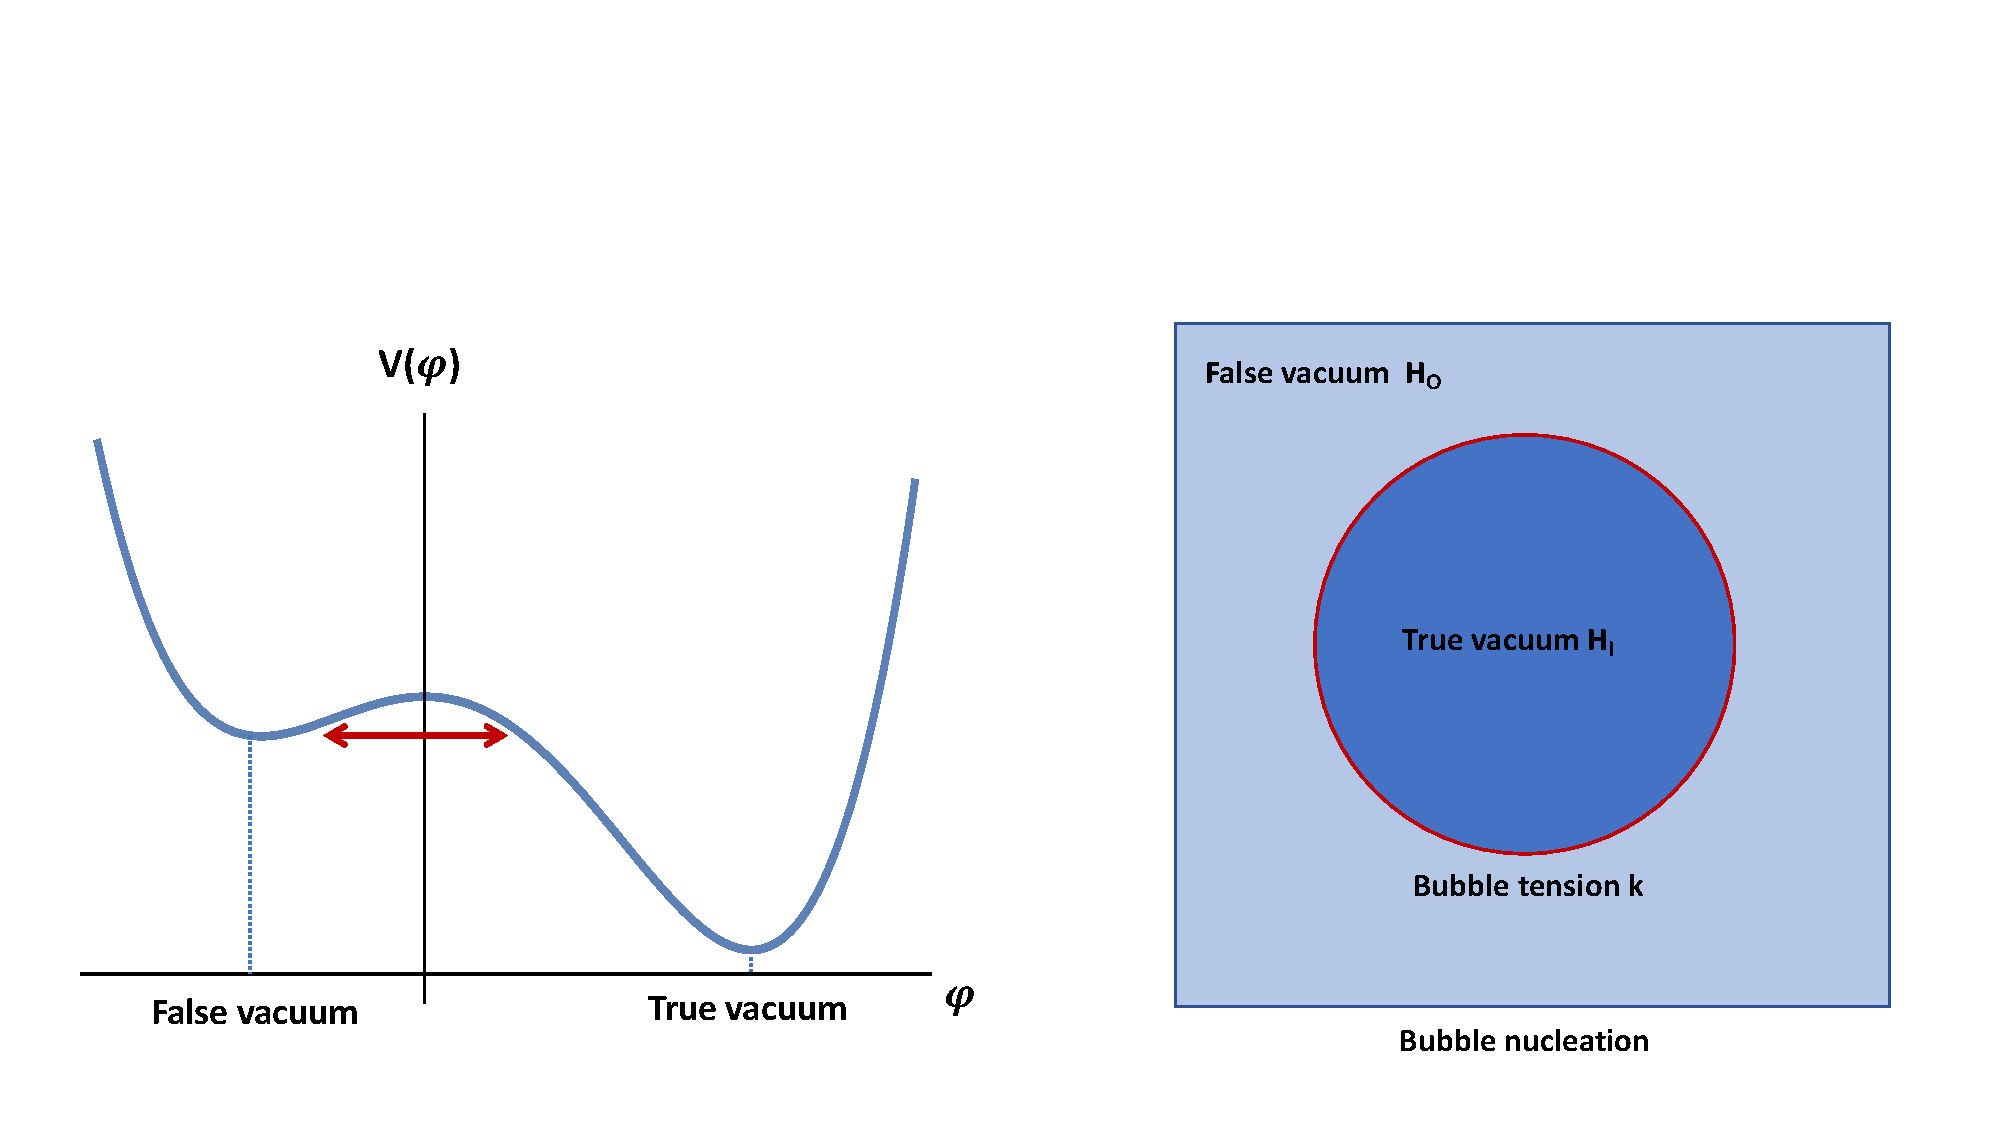
\includegraphics[width=120mm,height=72mm]{Sections/Figures/BubbleNucleation.pdf} 
\caption{Vacuum transitions in field theory and gravity.} \label{Fig:BN} 
\end{center}
\end{figure}

An important property of the bounce is that the field equations (and boundary conditions) are not only spherically symmetric, corresponding to the symmetry of the bubble, but have an enhanced $O(4)$ symmetry since they can be formulated in terms of the $O(4)$ invariant parameter $\xi^2= \tau^2+r^2$. Coleman and collaborators used an $O(4)$ ansatz $\varphi=\varphi(\xi)$ to find the bounce and later on proved that it is actually the minimum configuration \cite{Coleman:1977th}. However, in order to study the further evolution of the bubble after materialisation, a Wick rotation needs to be performed $\tau\rightarrow it$ and the $O(4)$ symmetry becomes $O(3,1)$. The region outside the light-cone of the origin can be properly treated in terms of the coordinates $t,r$. But the region inside the light-cone does not exist in the Euclidean coordinates and in Lorentzian coordinates are better described by the change of coordinates $(\hat t, \hat r)=(\sqrt{t^2-r^2}, r/\sqrt{t^2-r^2})$. It can be easily seen  that in terms of these coordinates the Minkowski metric takes the form
 \be
 ds^2=d\hat t^2- \hat t^2\left[\frac{d\hat r^2}{1+\hat r^2}+\hat r^2\left(d\theta^2+\sin^2\theta d\phi^2\right)\right]=d\hat t^2- \hat t^2 d\Omega^2_{(k=-1)}
 \ee
corresponding to a an open ($k=-1$) FLRW universe.

\subsubsection*{Transitions including gravity}

Let us then briefly review the subject of vacuum transitions in gravitational theories (also illustrated in figure \ref{Fig:BN}). Following the Euclidean approach, in a seminal contribution,  Coleman and de Luccia (CDL) \cite{Coleman:1980aw} further generalised the vacuum transition formalism  to include the effects of gravity. Contrary to the case without  gravity, in which the formation and evolution of the bubble corresponds to opposite contributions from internal pressure and the tension of the wall, once gravity is included it also contributes to the stability of the bubble. In particular it allows up-tunneling transitions from the true vacuum to the false vacuum in which pressure and tension both tend to compress the bubble but gravity, through the presence of the cosmological constant, contributes towards the expansion of the bubble. actually, Lee and Weinberg \cite{Lee:1987qc} estimated the transition rate from true to false vacuum.

A further important observation on the gravity case is that there is no proof that  the optimal instanton configuration is the $O(4)$ symmetric bounce. Nevertheless CDL assumed this symmetry and managed to estimate the transition rates for both dS to Minkowski and Minkowski to AdS. Further generalisations were done later on.

A related but different approach to vacuum transitions was performed by Brown and Teitelboim (BT) \cite{Brown:1988kg} in which instead of a scalar potential with different minima, they studied bubble nucleation in terms of a theory with fluxes, similar to the ones discussed in the previous sections. They concentrated on the case of 3-index antisymmetric tensors coupled to gravity in which even though they do not correspond to propagating degrees of freedom, they can give rise to the nucleation of membranes in 4 dimensions. A chain of transitions may be induced reducing the fluxes and then the value of the cosmological constant. Their estimate of the transition rates were performed in the Euclidean approach and agree with the CDL calculations in the thin wall approximation. In particular for a transition from dS space with cosmological constant $\lambda_{\rm O}=3H_{\rm O}^2$ to another vacuum with $\Lambda_{\rm I}=3H_{\rm I}^2$ nucleating a bubble of tension $\kappa$ is $\Gamma=e^{-B/\hbar}$ with 
\be
B  =-\frac{\pi}{G}\left[ \frac{\left[ (H_{{\rm O}}^{2}-H_{{\rm I}}^{2})^{2}+\kappa^{2}(H_{{\rm O}}^{2}+H_{{\rm I}}^{2})\right] R_{{0}}}{4\kappa H_{{\rm O}}^{2}H_{{\rm I}}^{2}}-\frac{1}{2}\left(H_{{\rm I}}^{-2}-H_{{\rm O}}^{-2}\right)\right] \label{eq:SdS}
\ee
where
\be
R_{0}^{-2}  =\frac{1}{4\kappa^{2}}\left[(H_{{\rm O}}^{2}-H_{{\rm I}}^{2})^{2}+2\kappa^{2}(H_{{\rm O}}^{2}+H_{{\rm I}}^{2})+\kappa^{4}\right]\label{eq:R0}\\
\ee
Here the indices I and O refer to inside and outside the bubble. This includes both down and up-tunneling between the 2 dS spacetimes. An interesting property of these transitions is that the ratio of up to down-tunneling can be easily computed and give $\Gamma_{\rm up}/\Gamma_{\rm down}=e^{-(S_{TV}-S_{FV})}$ with $S_{TV}, S_{FV}$ corresponding to the entropies of each of the vacua, true and false respectively. Recall that the entropy of dS space is given by $S=\pi/(GH^2)$. Therefore this is a statement of detailed balance in which in equilibrium the relative transition rates  are weighted by the corresponding entropy. Similar to the case without gravity, the evolution of the bubble after materialisation requires an analytic continuation from a Euclidean to a Lorentzian metric that describes an open universe. Note, however, that this result fully relied on the underlying $O(4)$ symmetry of the bounce, something which is far from being shown in the case with gravity.

Similar results for the transition rates hold for AdS down tunneling. However here a condition on the relative value of the cosmological constants and the wall tension has to be satisfied: 
$\kappa<\sqrt{|H_{\rm I}^2}-\sqrt{|H_{\rm O}^2|}$. Furthermore up-tunneling from AdS  is not allowed. Nor from Minkowski to dS. However a proposal by Farhi, Guth and Guven (FGG) \cite{Farhi:1989yr} for {\it creation of universes in the laboratory} meaning nucleating a dS bubble from Minkowski, has been considered. Following the standard Euclidean approach it was found that a singular instanton is needed in order to achieve the bubble nucleation. 

This prompted a Hamiltonian approach by Fischler, Morgan and Polchinski \cite{Fischler:1990pk} in which the Minkowski to dS transition was reconsidered and concluded that it is actually possible to realise the FGG proposal in Lorentzian spacetimes. A key ingredient of this Hamiltonian formalism is to assume only the standard $O(3)$ spherical symmetry to describe the bubble and its evolution. This symmetry automatically include Schwarzschild black holes solutions with a given mass parameter $M$. As long as $M\neq 0$ the up-tunneling from Minkowski is allowed. Recent generalisations of this result have been developed \cite{Bachlechner:2016mtp,DeAlwis:2019rxg}. The Hamiltonian approach is so far very much restricted to the extreme thin-wall approximation and further developments need to be performed to include scalar potentials with different minima. The calculations are also performed in the global dS slicing that when studying the further evolution of the bubble wall fits with a closed rather than open universe. This put at least into question the general claim from the Euclidean approach that the universe within the bubble has to correspond to an open universe. This is an important point for the string landscape since if the open universe claim holds in general, it may be conceivable to rule out the full string landscape if in the future is found that the universe is not open \cite{Dyson:2002pf, Freivogel:2005vv, Cespedes:2020xpn}. This subject needs further studies before arriving to a concrete conclusion. 

\subsubsection*{Transitions in string scenarios}

\begin{figure}[t]
\begin{center}
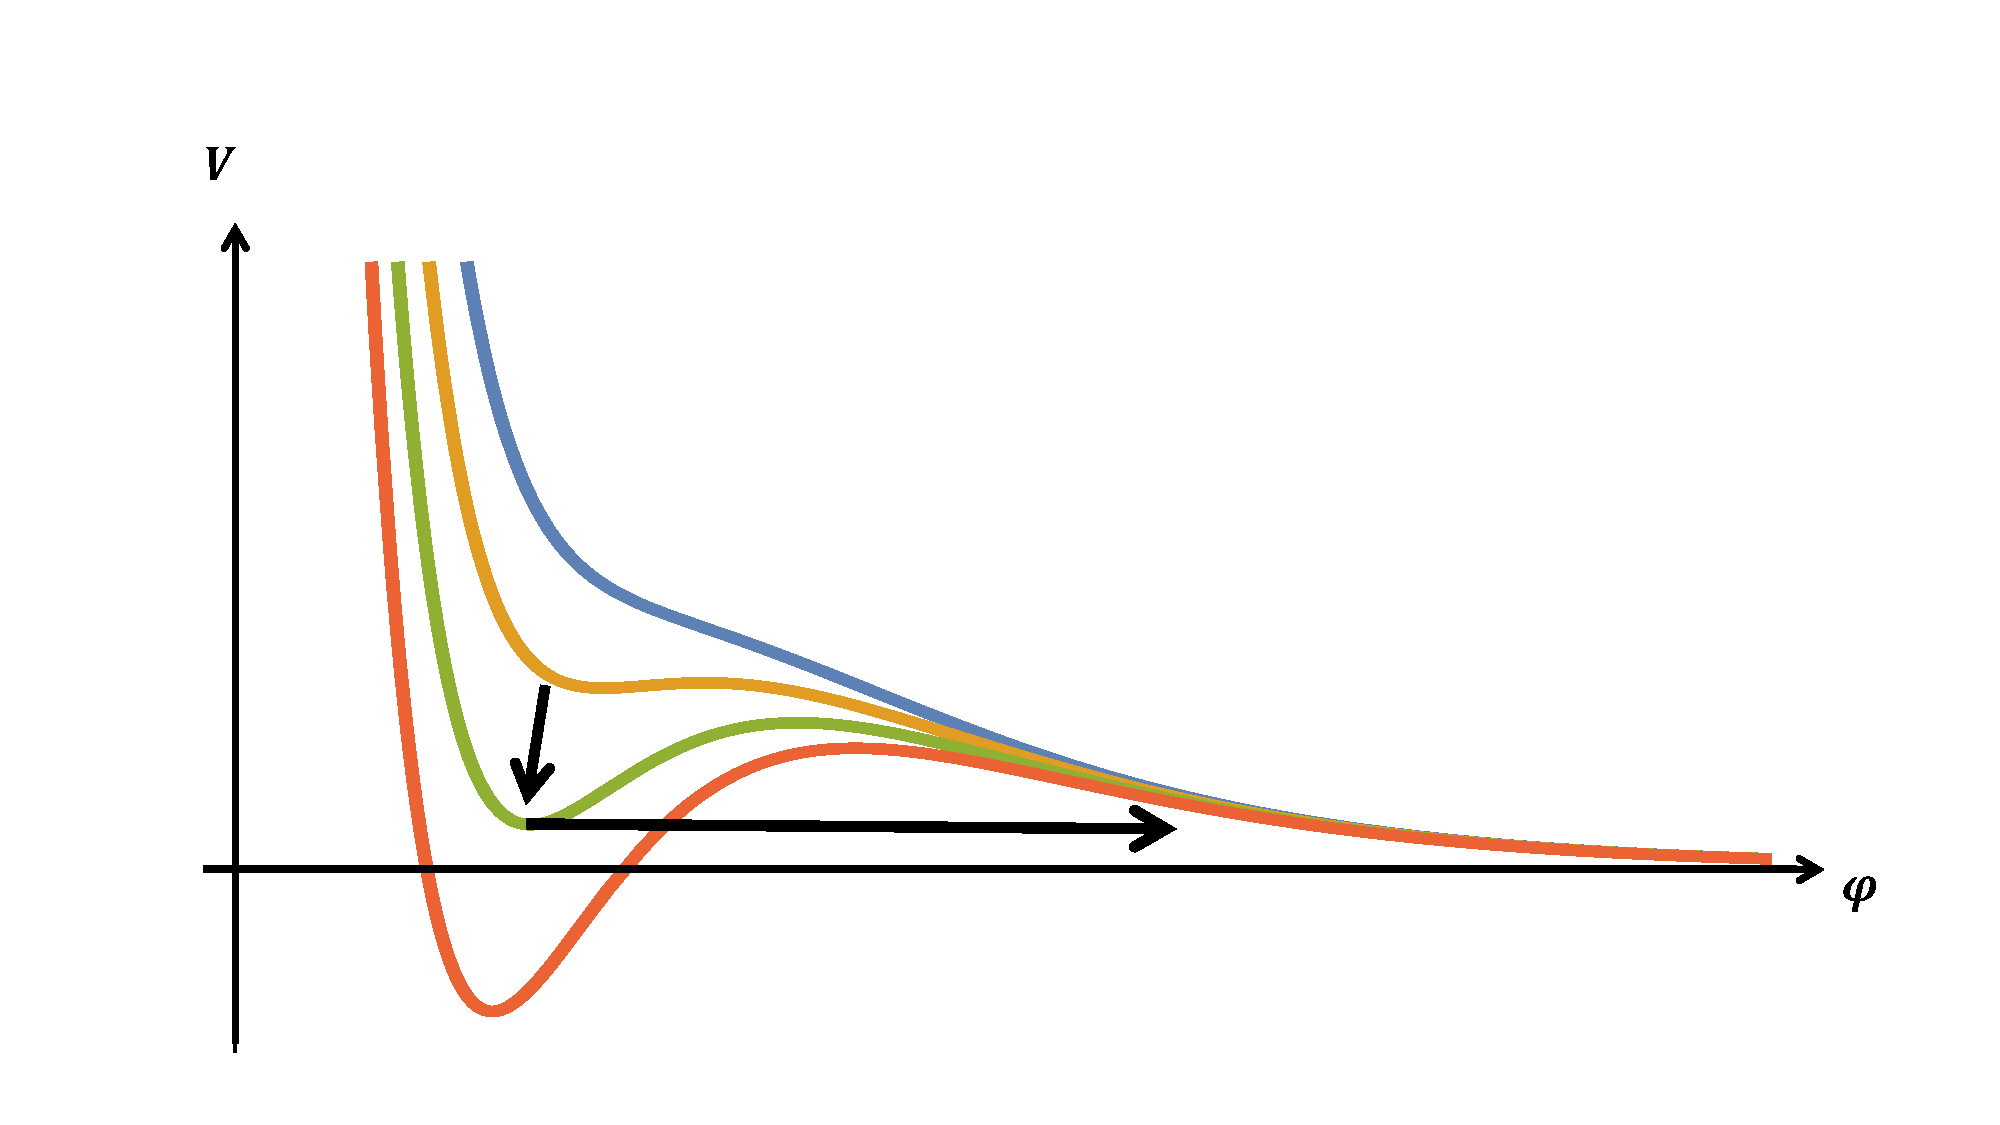
\includegraphics[width=120mm,height=72mm]{Sections/Figures/VacuumTransition0.pdf} 
\caption{Vacuum transitions in string theory. First bubble nucleation from flux/D3 brane charge transitions illustrated by the vertical arrow. Then a CDL-like transition crossing the potential barrier illustrated by the horizontal line. In string theory this transition may correspond towards decompactification.} \label{Fig:BN2} 
\end{center}
\end{figure}
In string theory (illustrated in figure \ref{Fig:BN2}) we may consider the scenarios discussed in the previous sections. First we should point out that there can be at least two different types of transitions:
\begin{enumerate}
\item
Transitions of the Brown-Teitelboim type corresponding to transitions among vacua corresponding to the different quantised fluxes. Concretely, given two vacua with values of three-form fluxes 
$H_{mnp}$, $F_{mnp}$ in terms of integers $(K,M)$. For a transition from a $(K,M)$ vacuum to a $(K',M')$ vacuum, a brane carrying D3-brane charges $(K-K',M-M')$ can be nucleated to mediate between the two vacua. These are precisely D5 (or NS5 ) branes that can wrap the 3-cycles carrying the fluxes and with the remaining 2 spatial dimensions corresponding to an $S^2$ wall separating the two different 4-dimensional vacua.  

This provides an elegant string theory implementation of the 4-dimensional vacuum nucleation picture. It fits nicely in the sense that D3 and D7 branes being BPS and codimension 4 have been used to host the Standard Model and/or hidden sectors, whereas D5-branes do not play a direct role as long as supersymmetry is preserved (since supersymmetry requires codimension 4 branes). But D5-branes naturally couple to 3-forms and furthermore the extra dimensions nicely fit with the dimension of a wall separating different 4-dimensional vacua. From the 4-dimensional EFT, there is not a scalar potential which connects the two vacua so this cannot be explicitly described in terms of the CDL bounce solution within the 4-dimensional EFT. But it fits nicely in the BT formalism.

\item Transitions {\it a la}  CDL are also implemented since any potential dS vacuum should coexist with the runaway vacuum corresponding to infinite volume and vanishing string coupling. The potential for the volume modulus connects both vacua and the transition may be estimated.
\end{enumerate}

Transition rates have been estimated for type IIA \cite{Narayan:2010em} as well as type IIB flux compactifications  (for both KKLT and LVS) vacua \cite{Kachru:2003aw, Westphal:2007xd, deAlwis:2013gka}. The probability amplitude $\Gamma\sim e^{-24\pi^2/\Lambda_0}$ where $\Lambda_0$ is the value of the scalar potential at the dS minimum. The corresponding lifetime $\tau \sim 1/\Gamma$ is exponentially small as compared with the Poincar\'e recurrence time which is reassuring. Furthermore the transition from dS to an AdS is preferred over dS to dS and the CDL transition towards decompactification dominates the dS to dS transitions.

An interesting observation was made in \cite{Johnson:2008vn,Aguirre:2009tp} regarding the actual implementation of the bounce solution in a toy model version of flux compactifications with two dS vacua plus the runaway. The claim is that not only the decompactification transition is preferred but that the potential bounce solution connecting the two dS vacua necessarily follows into the runaway towards decompactification providing a potential  obstacle to implement the transition. Note however that contrary to the toy model in which both transitions  corresponded to the CDL type, in flux compactifications the flux transition is of the BT type whereas the decompactification is of the CDL type.

\enddocument

\newpage